\chapter{Machine Learning}

Consideremos un conjunto de datos $X = (x_1, \dots , x_N)$ donde para cada $i \in {1, \dots, N}$, $x_i = [x_{i}^1 , \dots, x_{i}^M]$ es decir, un conjunto de $N$ datos con $M$ features cada uno. Consideremos además $Y = (y_1, \dots , y_N)$ las etiquetas o labels cada cada dato. En problemas de clasificación binario, $y_i \in \{ 0, 1\}$ y en problemas de clasificación multiclase, $y_i \in \{1, \dots L\}$. Para problemas de regresión, $Y = (y_1, \dots , y_N)$ con cada $y_i \in \mathbb{R}$.

\section{Linear Regression}

Un modelo de regresión lineal es un modelo de aprendizaje \textbf{supervisado} utilizado para problemas de \textbf{regresión} y \textbf{clasificación}. Se construye a través de la búsqueda de parámetros $\beta_0, \dots, \beta_M$ que multiplican el input para obtener la predicción. En problemas de regresión, 
$$\hat{y} = f(\beta) = \beta_0 + \sum_{j=1}^M \beta_j x^j$$
y en problemas de clasificación a través de una función sigmoide 
$$\hat{y} = f(\beta) = \frac{1}{1+e^{- (\beta_0 + \sum_{j=0}^M \beta_j x^j)}}$$.

\begin{figure}[H]
    \center
    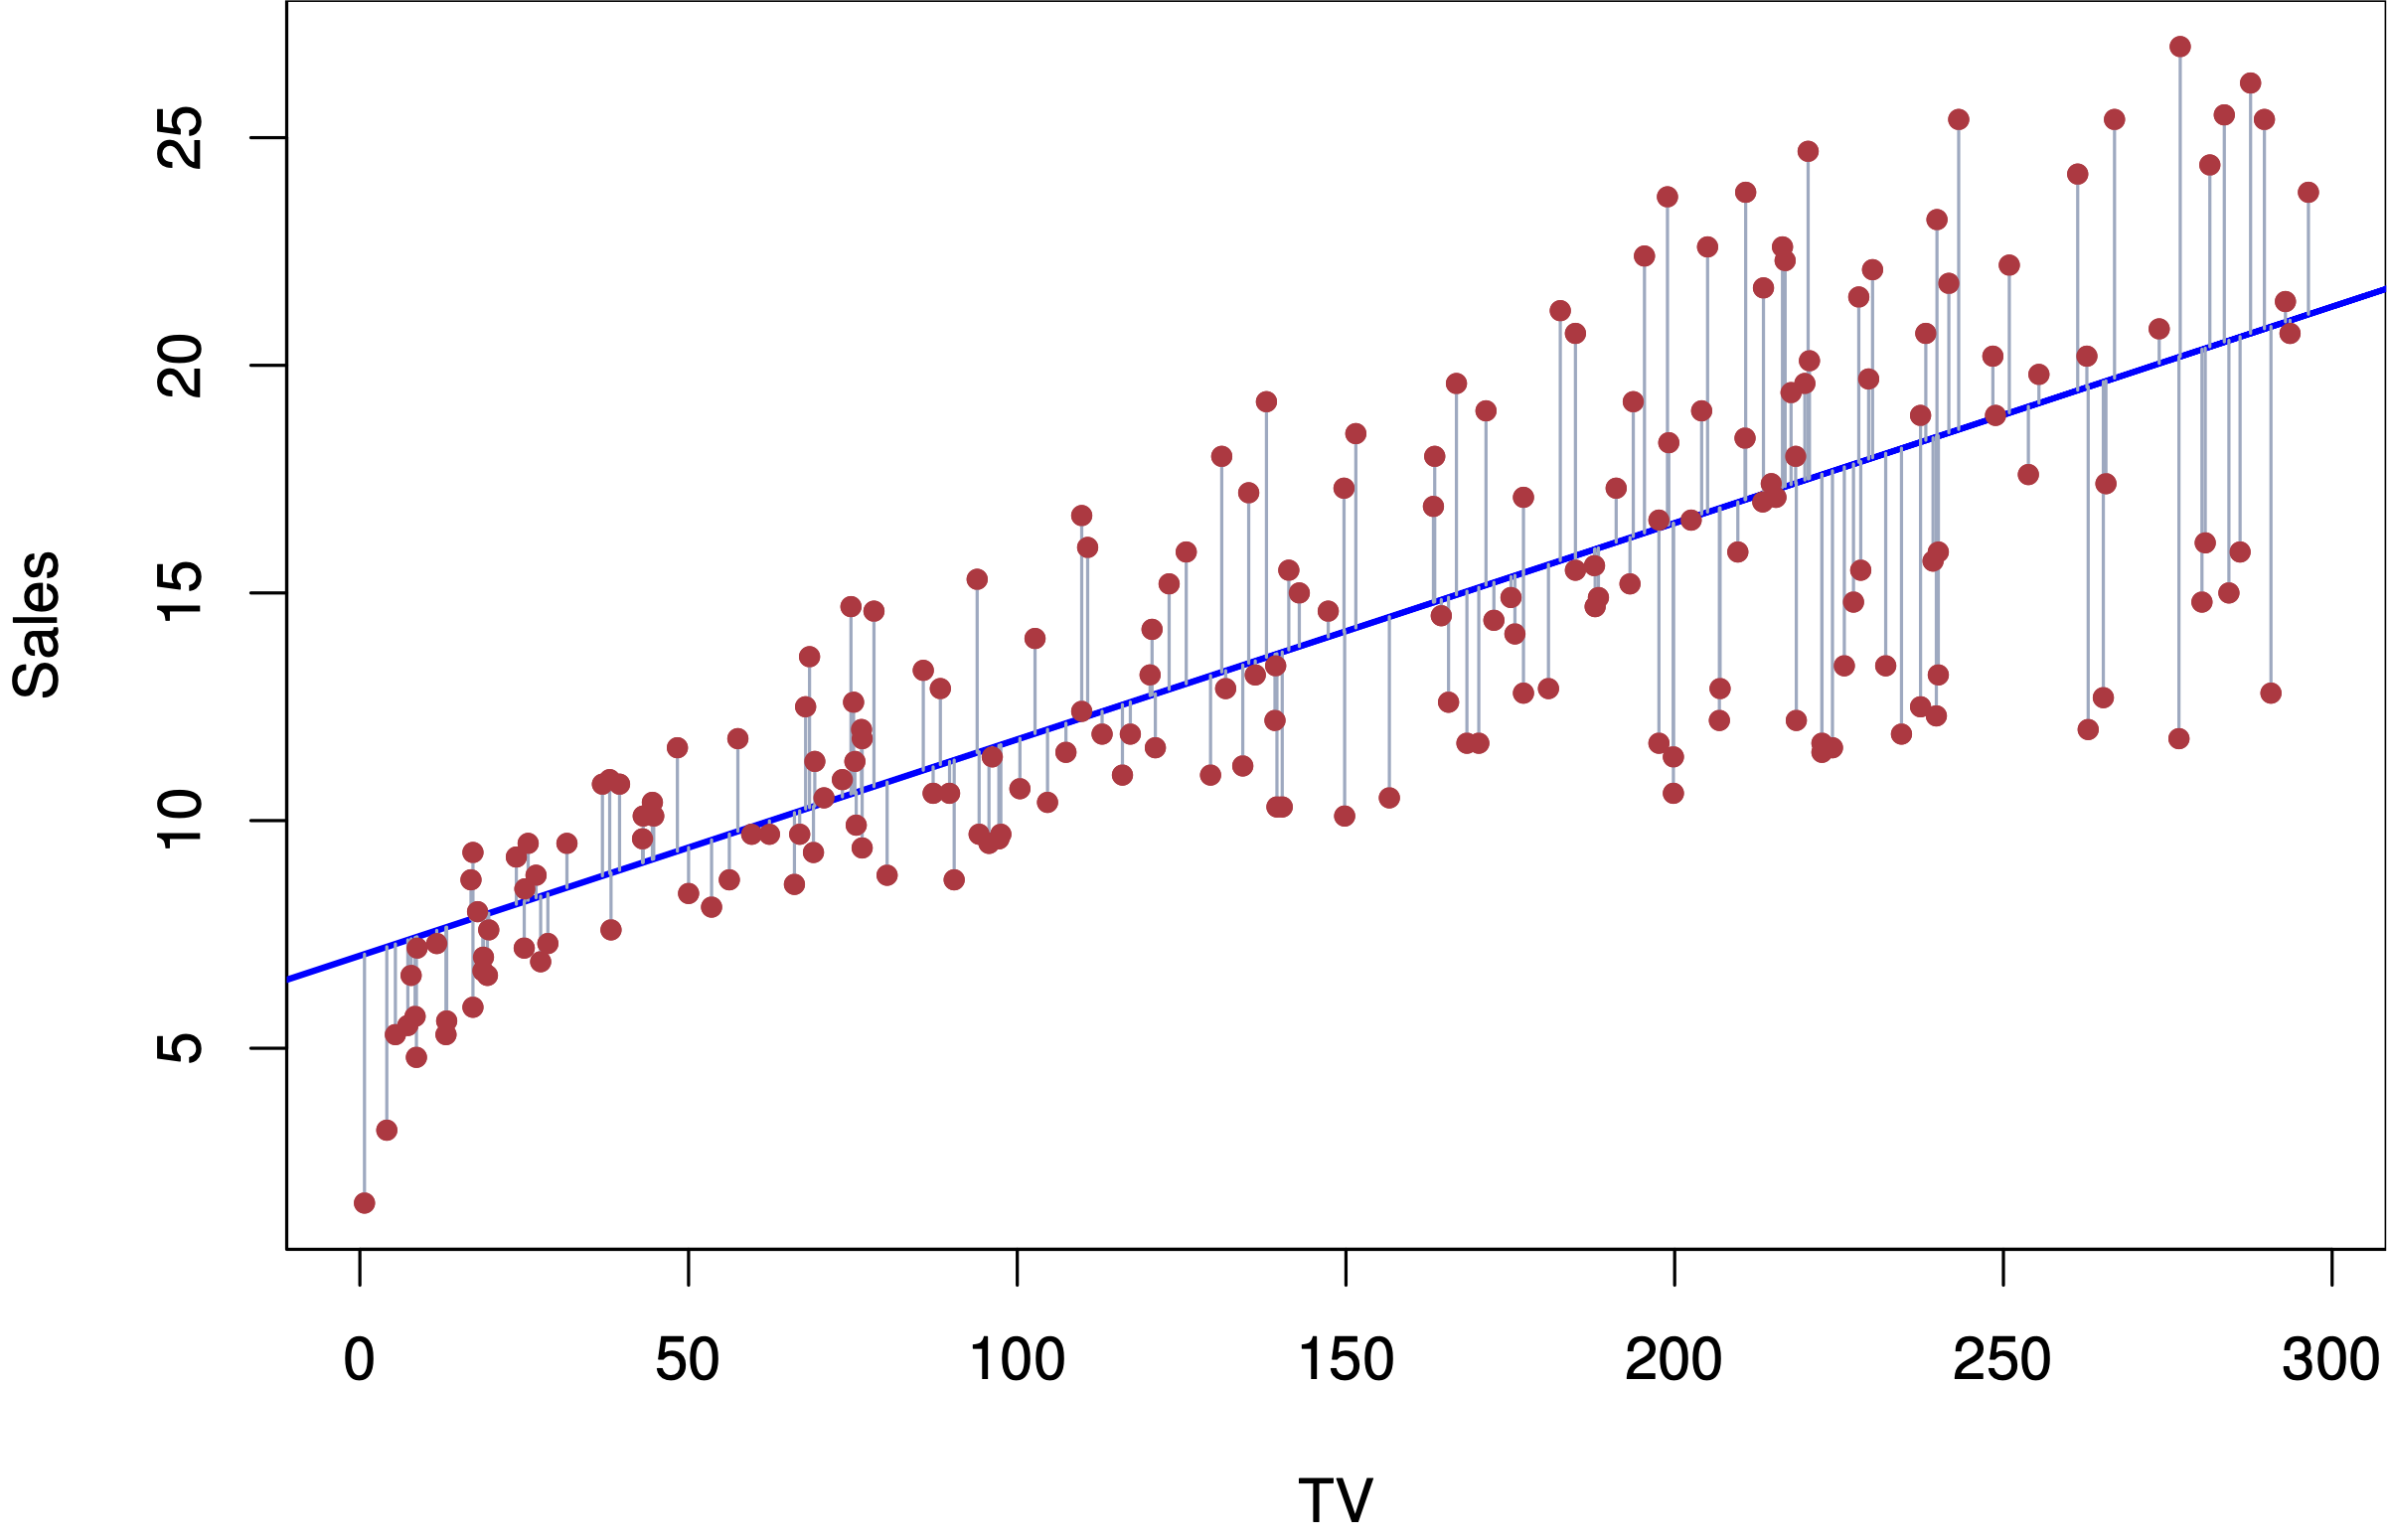
\includegraphics[scale=0.5]{notebooks/ML/img/linear_regression_diagram.png}
    \caption{Linear Regression Diagram}
\end{figure}

El problema a optimizar (mínimos errores cuadrados) queda entonces definido por 
$$\min_{\beta} \quad \frac{1}{N}\sum_{i=1}^N(y_i - f(\beta))^2$$
Cuya solución es cerrada en el caso de estimar una regresión y estimada a través del descenso de gradiente en el caso de una clasificación. 

\subsection{Regularization}

Para prevenir el overfitting y que la importancia de los parámetros quede mejor distribuida, es posible agregar a la función un término regularizador de la siguiente forma

\begin{equation*}
\begin{aligned}
\min_{\beta} \quad \frac{1}{N}\sum_{i=1}^N(y_i - f(\beta))^2 \\
\textrm{s.t.} \quad ||\beta||^{p}_{p} \leq t
\end{aligned}
\end{equation*}

De manera equivalente, por el método de \textit{Lagrange}, sin optimizar el valor de $\lambda$ y eliminando constantes que no dependen de $\beta$
$$\min_{\beta} \quad \frac{1}{N}\sum_{i=1}^N(y_i - f(\beta))^2 + \lambda ||\beta||^{p}_{p}$$
Cuando $p=1$ se le conoce como regresión \textbf{Lasso} y cuando $p=2$ una regresión \textbf{Ridge}. La combinación de ambas restricciones es conocida como \textbf{Elastic Net}. 

\begin{figure}[H]
    \center
    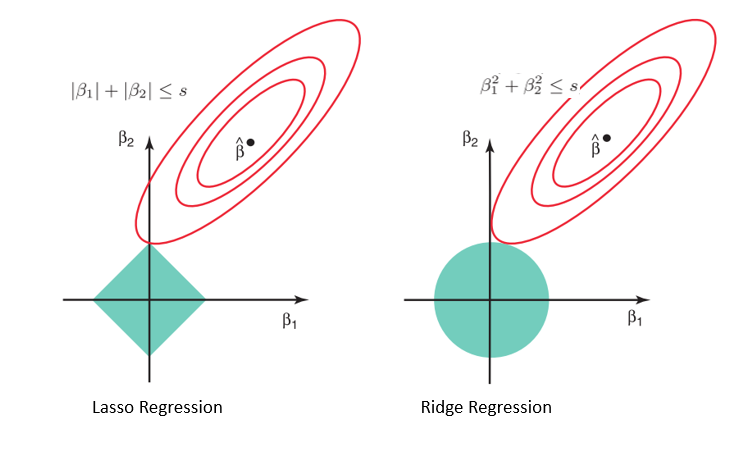
\includegraphics[scale=0.4]{notebooks/ML/img/lasso_and_ridge_diagram.png}
    \caption{Lasso and Ridge Diagram}
\end{figure}

Notar que la restricción para el caso \textit{Lasso} hace más probable que las curvas de nivel intersecten la restricción en una esquina (en mayor dimensión es incluso más probable) por lo que los parámetros que no son importantes para el modelo, serán llevados a 0. En el caso de la restricción \textit{Ridge}, la forma permite que los valores queden acotados pero ninguno será llevado a 0.

\begin{figure}[H]
    \center
    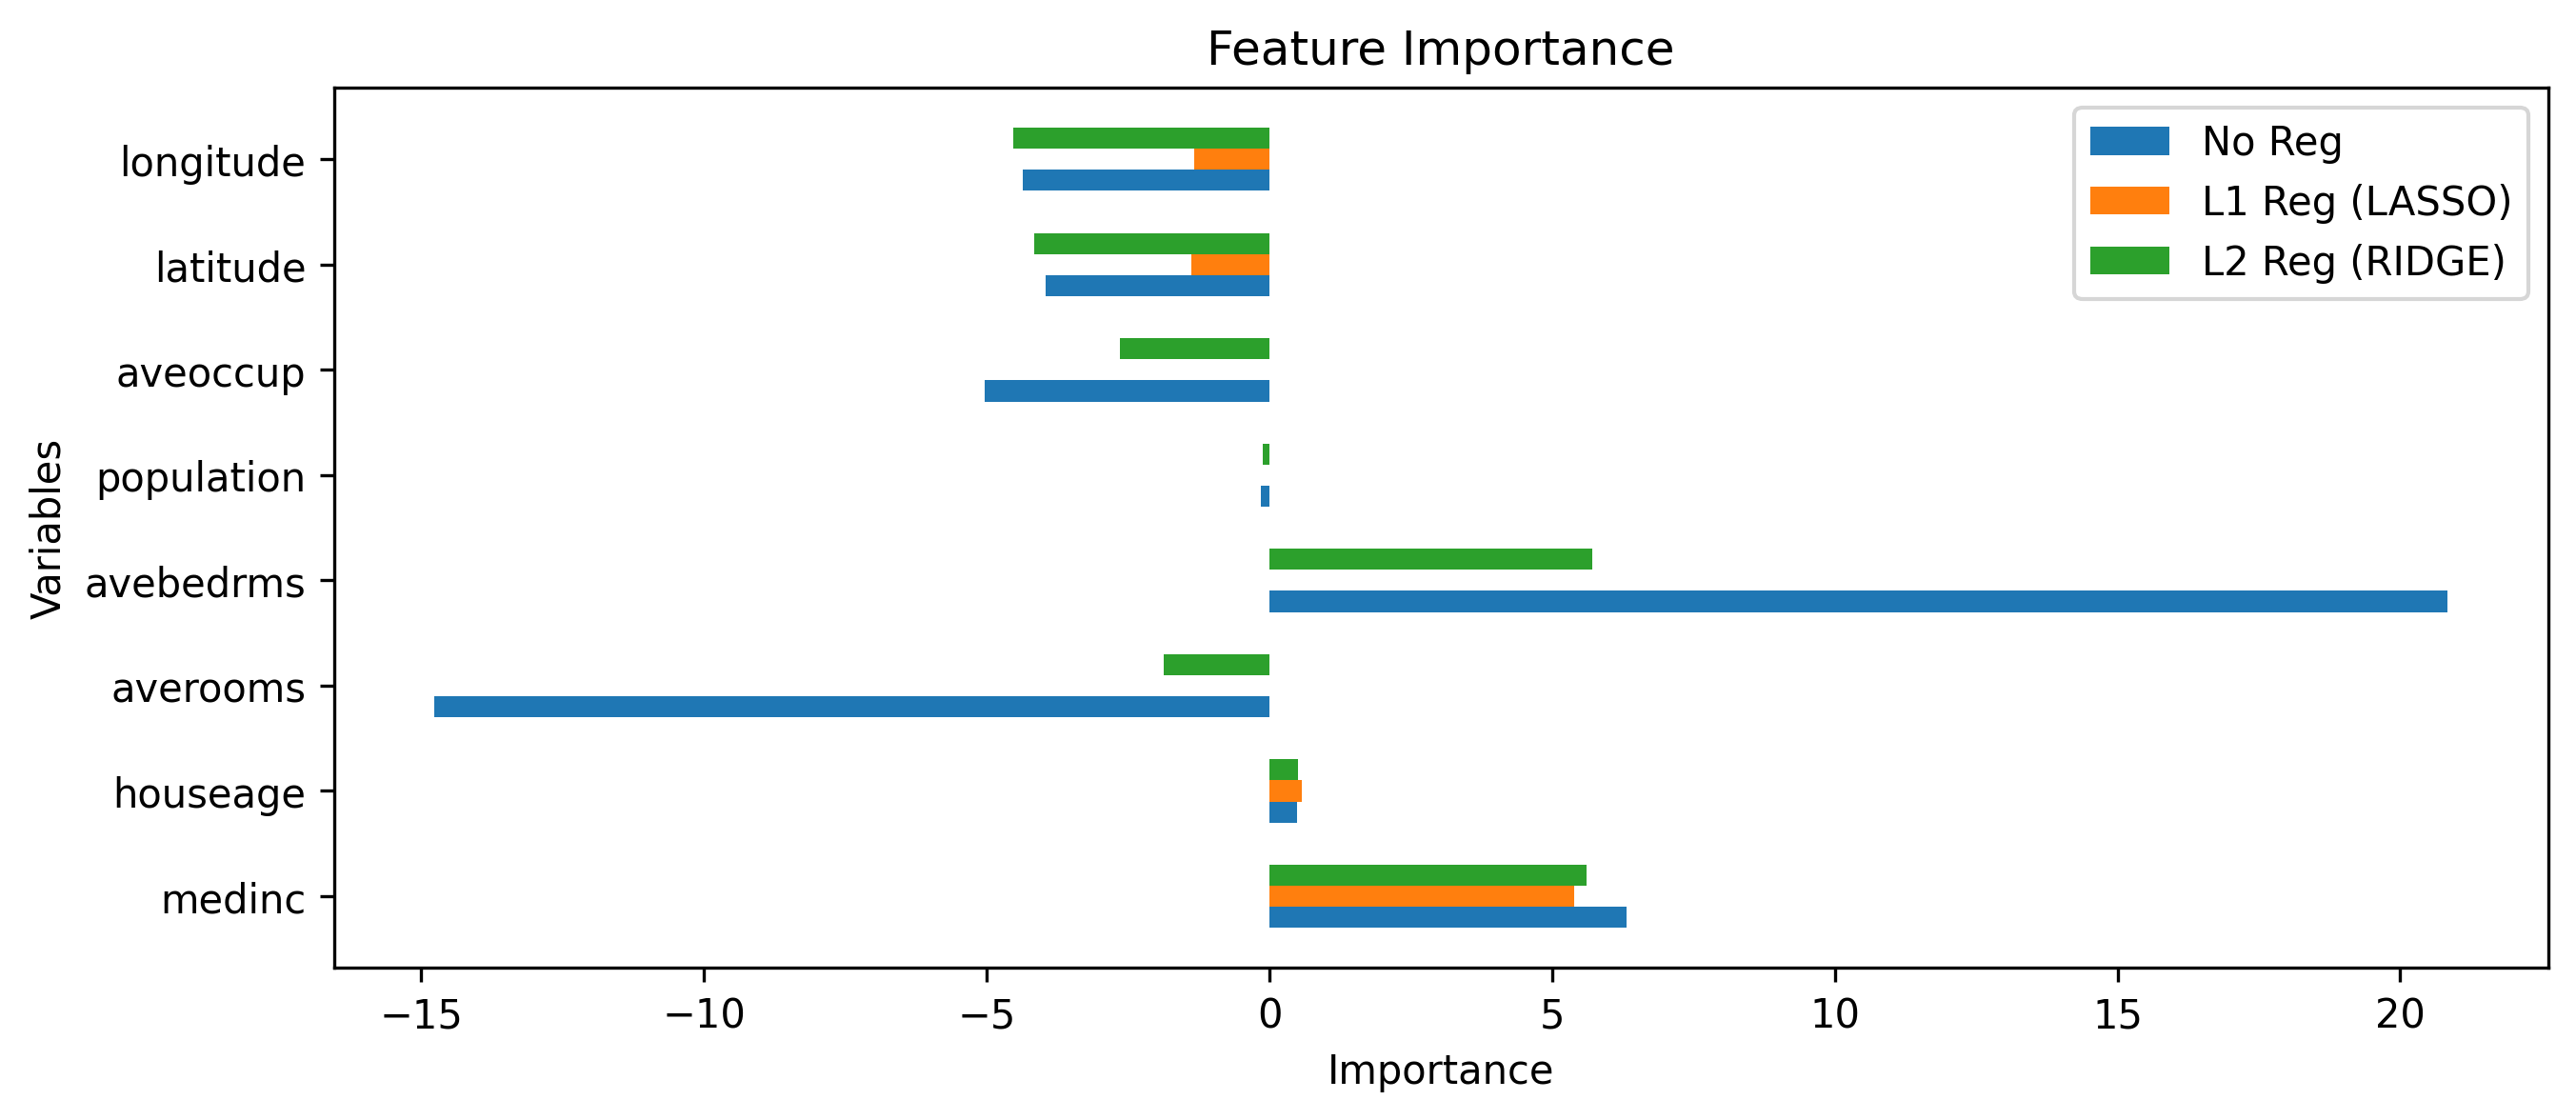
\includegraphics[scale=0.5]{notebooks/ML/img/regularization_feature_importance.png}
    \caption{Regularization Feature Importance}
\end{figure}


\section{Decision Trees}

Un árbol de decisión es un modelo de aprendizaje \textbf{supervisado} utilizado para problemas de \textbf{regresión} y \textbf{clasificación}. El objetivo es aprender simples reglas de decisión a partir de las features. 

\begin{figure}[H]
    \center
    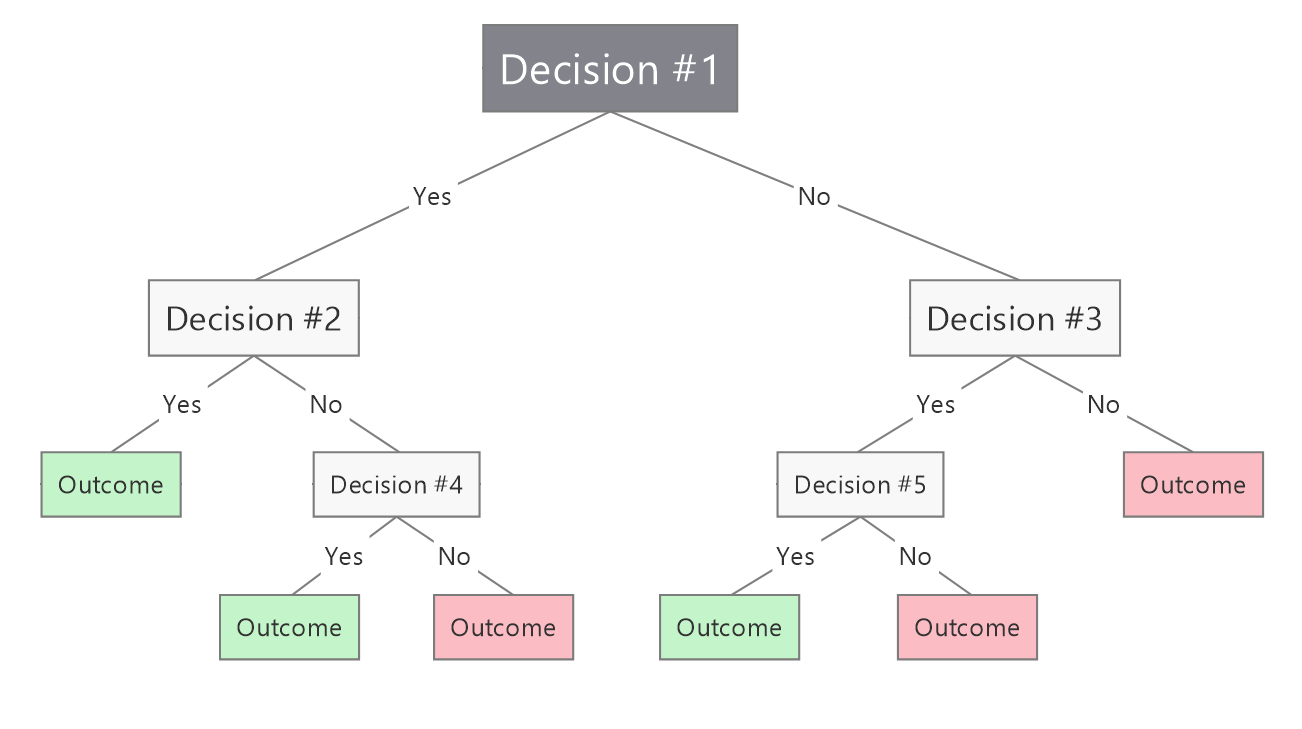
\includegraphics[scale=0.25]{notebooks/ML/img/decision_tree_diagram.png}
    \caption{Decision Tree Diagram}
\end{figure}

En el caso de un problema de clasificación, la variable a escoger y el corte correspondiente se puede elegir como aquel que minimice el desorden de los elementos. Definimos primero la \textbf{entropía} según 
$$H(p) = - \sum_{j=1}^{L}p_j\log_{2}p_j$$

donde $p_j$ es la frecuencia relativa del label $j$ en un grupo. Notar que la entropía es mínima cuando el grupo solo tiene elementos de la clase 0 o de la clase 1 ($p_j = 1$) y máxima cuando hay la misma cantidad de elementos de cada clase ($p_j = \frac{1}{2}$). 

\begin{figure}[H]
    \center
    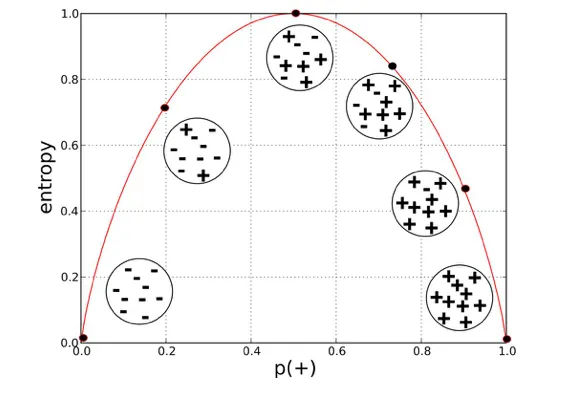
\includegraphics[scale=0.3]{notebooks/ML/img/entropy_diagram.png}
    \caption{Entropy Diagram}
\end{figure}

Con la entropía ya definida, definamos la \textbf{Information Gain} como 
$$IG(S,D) = H(S) - \sum_{V \in D}\frac{|V|}{|D|}H(V)$$

Donde el primer término es la entropía antes del split y el segundo término es la suma de las entropías después del split. Podemos iterar hasta que la \textit{Information Gain} no tenga modificaciones (es decir, llegar a los nodos puros) pero esto podría traer problemas de overfitting, en general esto se regula con la profundidad del árbol y escogiendo en cada iteración, la división que maximiza el IG. 

\begin{figure}[H]
\begin{subfigure}{.5\textwidth}
    \center
    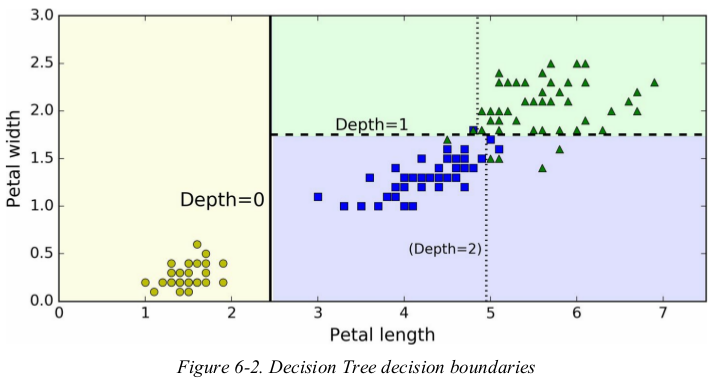
\includegraphics[scale=0.3]{notebooks/ML/img/decision_tree_data.png}
    \caption{Decision Tree Boundaries}
\end{subfigure}%
\begin{subfigure}{.5\textwidth}
    \center
    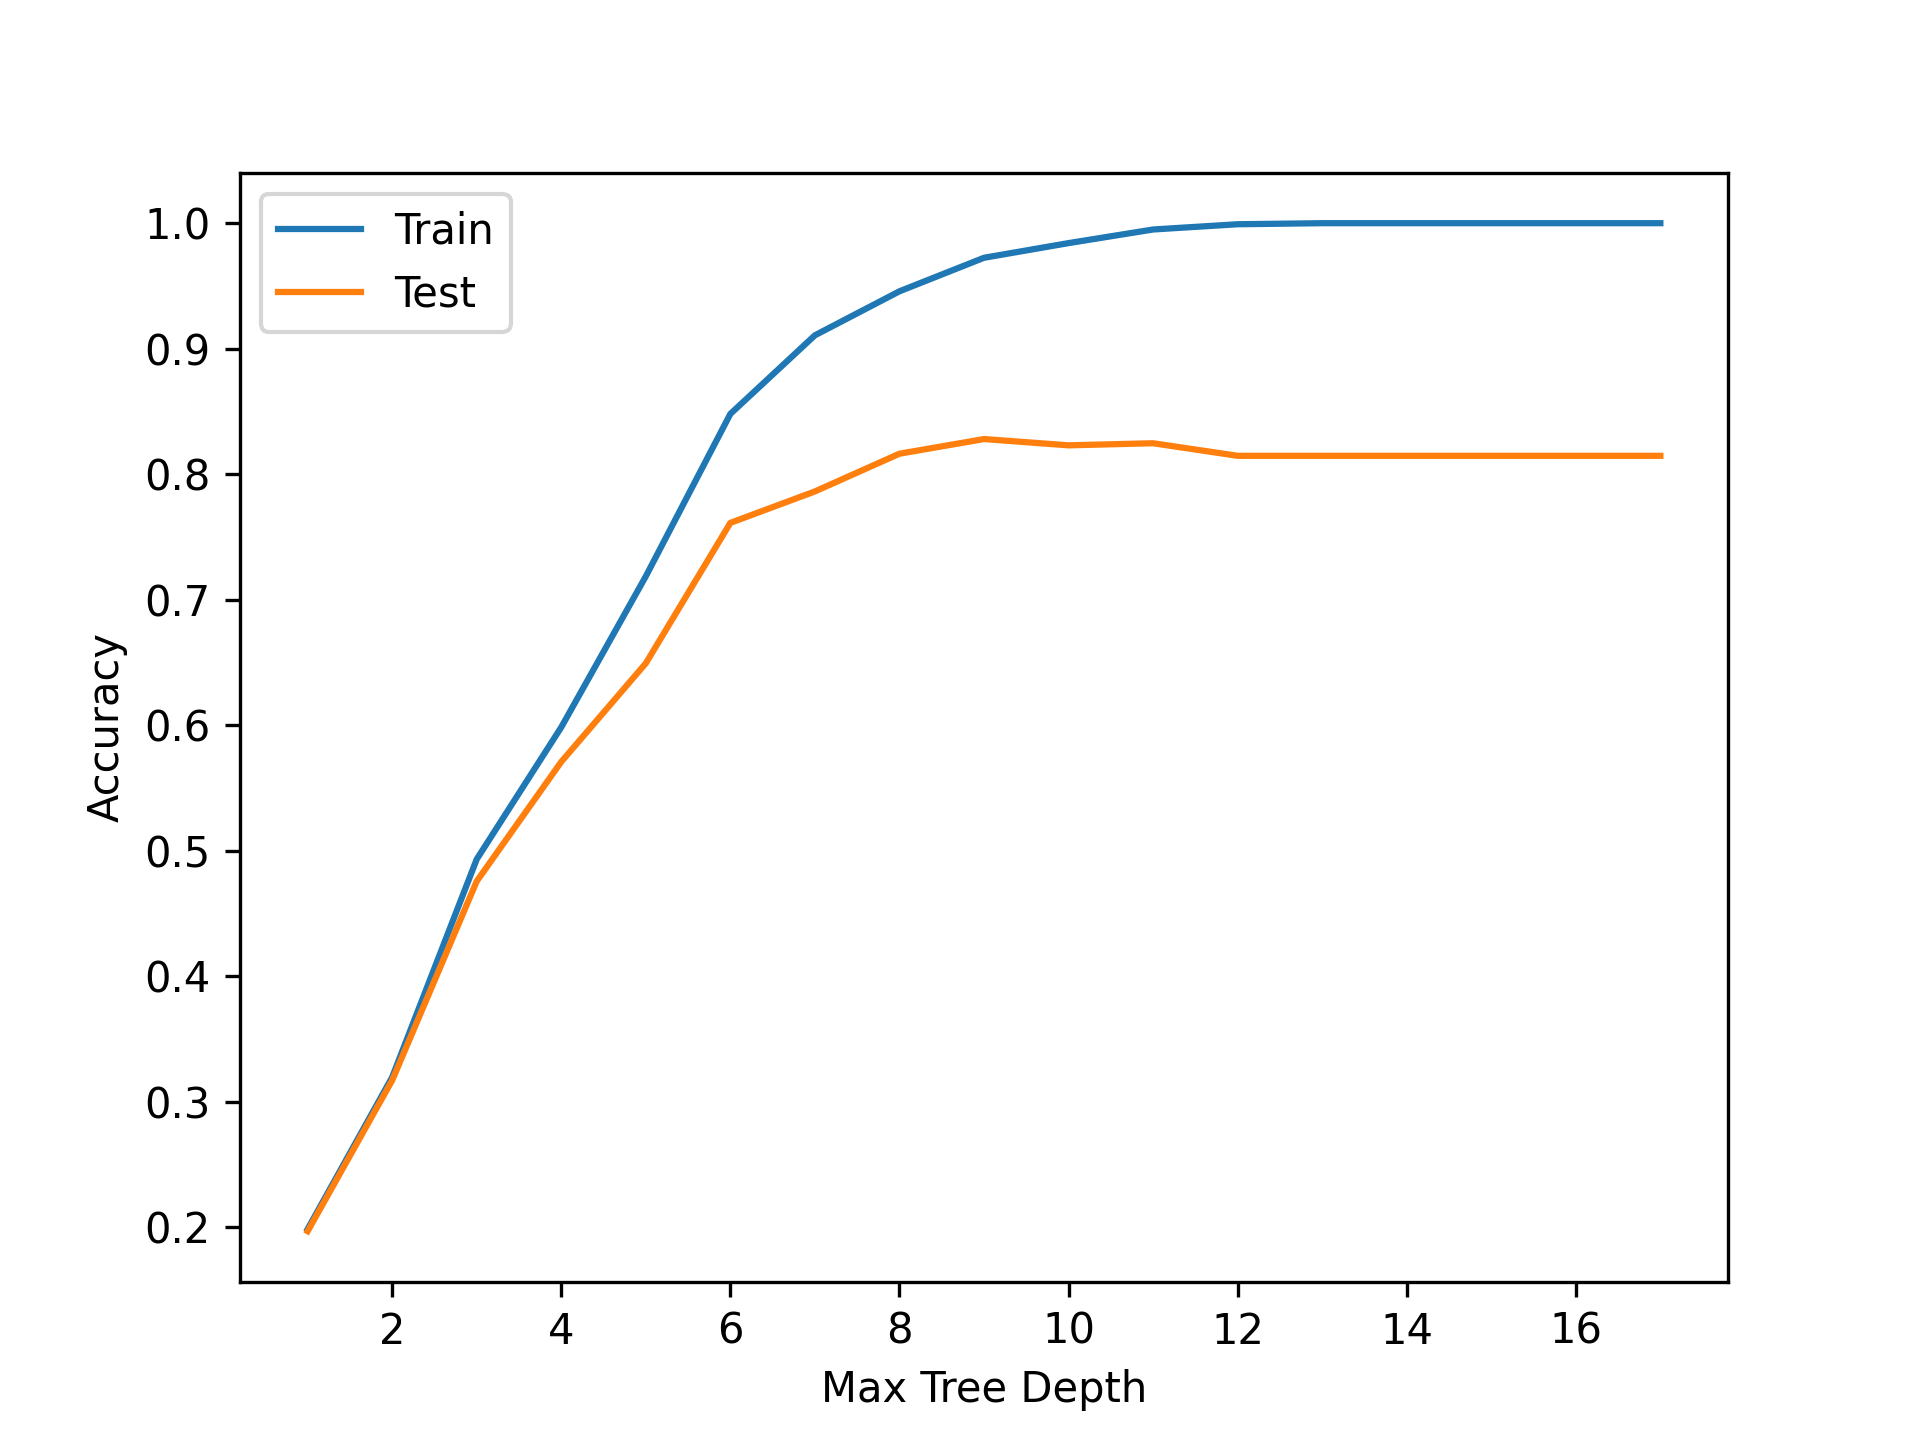
\includegraphics[scale=0.4]{notebooks/ML/img/max_depth_decision_tree.png}
    \caption{Max Depth and Accuracy}
\end{subfigure}
\caption{Decision Tree Implementation}
\label{fig:fig}
\end{figure}

En vez de la entropía, es posible usar otro indicador como el \textbf{Gini Index} definido como: 
$$G(p) = 1 - \sum_{j=1}^L p_j^2$$

\section{Random Forest}

\subsection{Ensemble Methods}

Los \textbf{métodos de ensamblaje} son aquellos en los que se combinan múltiples estimadores entrenados sobre los datos para generar una predicción más robusta (menor varianza) y generalizada. La predicción final se puede realizar por \textit{Majority Voting}, \textit{Simple Average} o \textit{Weighted Average}.

Existen 3 estrategias principales en los métodos de ensamblaje: 
\begin{enumerate}
    \item \textbf{Bagging}: Corresponde a una abreviación de \textit{Bootstrap Aggregating}, esta estrategia entrena cada estimador base con una \textbf{muestra con reemplazo} de ejemplos del conjunto de entrenamiento. (\textbf{Reduce la varianza})
    \item \textbf{Boosting}: Esta estrategia se basa en entrenar secuencialmente estimadores base débiles que \textbf{aprenden de los errores del anterior} para crear un estimador robusto. (\textbf{Reduce el bias})
    \item \textbf{Stacking}: Este método combina las predicciones de múltiples estimadores fuertes en una sola. 
\end{enumerate}

\begin{figure}[H]
    \center
    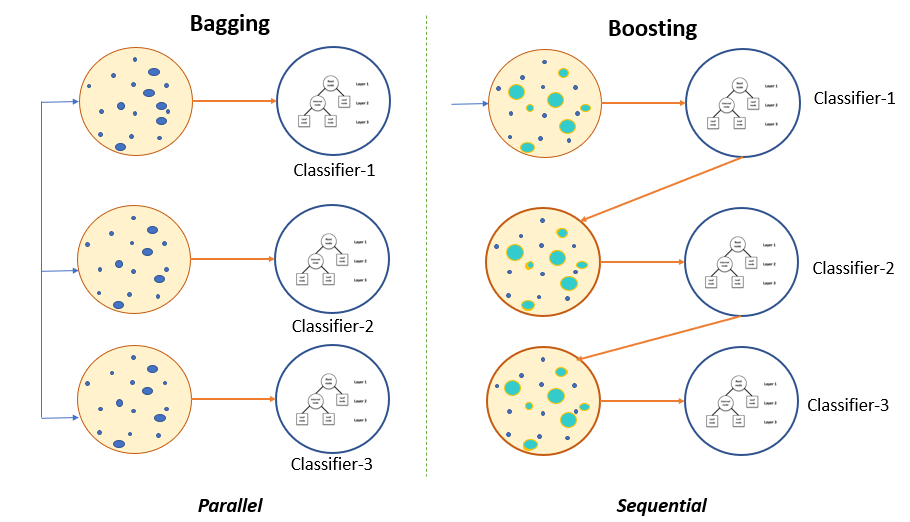
\includegraphics[scale=0.25]{notebooks/ML/img/bagging_and_boosting_diagram.png}
    \caption{Bagging and Boosting Diagram}
\end{figure}


El algoritmo de \textit{Random Forest} es un método \textbf{supervisado de ensamblaje} basado en \textit{Decision Trees}. Este, utiliza la estrategia de \textbf{bagging} para entrenar cada árbol de decisión sobre muestras con reemplazo del conjunto de entrenamiento y además, cada árbol es entrenado sobre un \textbf{subconjunto aleatorio de features} para asegurar que no haya similitud entre ellos. Ambas estrategias permiten mejorar la precisión del modelo y controlar el overfitting.

\begin{figure}[H]
    \center
    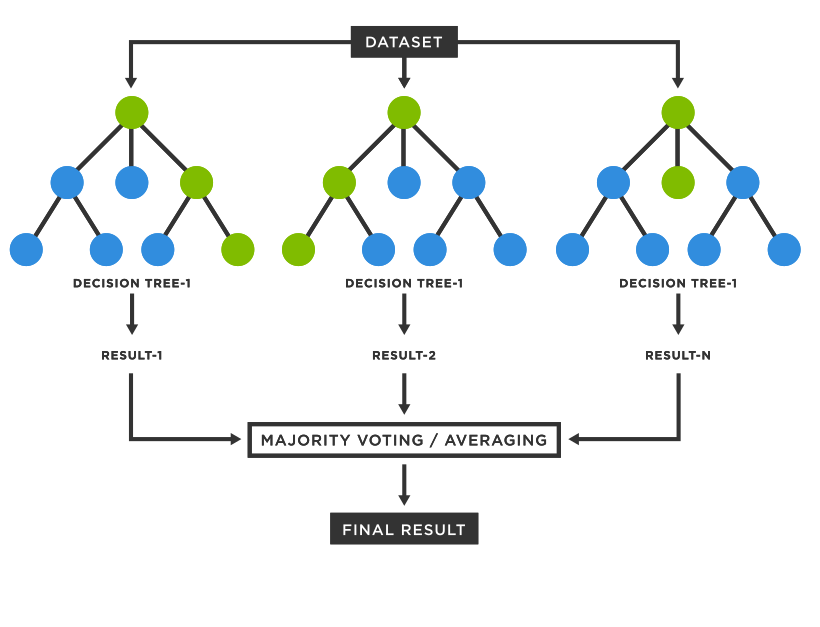
\includegraphics[scale=0.25]{notebooks/ML/img/random_forest_diagram.png}
    \caption{Random Forest Diagram}
\end{figure}

Para estimar la \textbf{feature importance} en modelos basados en árboles, se pueden mirar 3 posibles aspectos: 
\begin{enumerate}
    \item Suma de las \textit{information gain} con una variable determinada (o cuánto reduce la entropía, es equivalente). 
    \item Cantidad de nodos resultantes de la división con esa variable. 
    \item Profundidad promedio de un árbol en que su primera división es con esa variable. 
\end{enumerate}

Para extender esto a \textit{Random Forest}, se toma un promedio entre los distintos árboles de decisión que lo conforman. 

\section{Gradient Boosting Algorithm}

Los modelos de \textit{Gradient Boosting} son algoritmos basados en árboles que pueden ser utilizados para problemas de \textbf{clasificación y regresión}. 

\begin{figure}[H]
    \center
    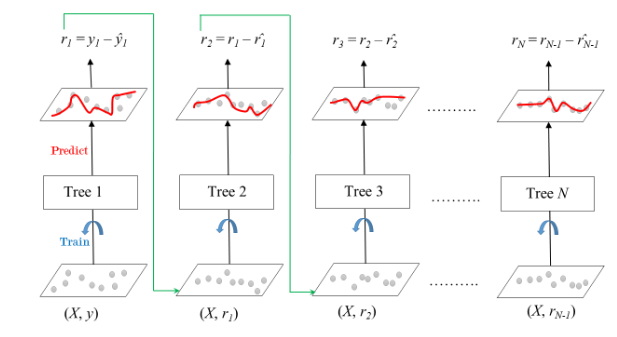
\includegraphics[scale=0.5]{notebooks/ML/img/gbc_diagram.png}
    \caption{Gradient Boosting Diagram}
\end{figure}

El entrenamiento consta en el aprendizaje secuencial de árboles de baja complejidad (\textit{weak learners}) que aprenden de los errores del anterior, vale decir, que aprenden en el conjunto de los \textbf{residuos} del modelo anterior. Sea $L(y , F(x))$ el error de la predicción del modelo $F(x)$ y el valor real $y$. 

El modelo $F(x)$ es el resultado de una combinación lineal de \textit{weak learners} tal que 
$$ 
F(x) = \sum_{k=1}^T \gamma_k h_k(x)
$$
Donde T es la cantidad de árboles (\textit{n estimators}), $h_k$ los  \textit{weak learners} y $\gamma_k$ su peso. Iniciando en un modelo inicial $F_0(x)$ entrenado sobre los datos, cada iteración se encarga de construir $F_{k}(x)$ según 
$$ 
F_{k} = F_{k-1} + \gamma_{k}h_{k}
$$
Para encontrar los valores $\gamma_{k} , h_{k}$ se siguen los siguientes pasos: 
\begin{enumerate}
    \item Calcular los residuos $i$ en la iteración $k$ como $r_{i,k} = - \left [ \frac{\partial L(y_i, F(x_i))}{\partial F(x_i)} \right ]_{F(x) = F_{k-1}(x)}$. En el caso de $L$ una función de error MSE, $r_{i,k} = 2(y_i - F_{k-1}(x_i)) \propto y_i - F_{k-1}(x_i)$
    \item Entrenar un \textit{weak learner} sobre $(X, r)$.
    \item Encontrar el valor de $\gamma_k$ como aquel que resuelve 
    $$ 
    \gamma_k = \argmin_{\gamma}\sum_{i=1}^N L(y_i , F_{k-1} + \gamma h_{k}(x_i))
    $$
    \item Hacer update al modelo según $F_{k} = F_{k-1} + \gamma_{k}h_{k}$
\end{enumerate}

La importancia de las variables es medida de manera similar a un \textit{Random Forest}, a través de la suma ponderada de las \textit{Information Gain} (o bien de la disminución de la entropía) que cada una de las features provoca en los distintos árboles. 

Existen otras formas de calcular la importancia de las variables, lo cual se discute en la sección \ref{subsec:shap_values}.

\section{Naive Bayes}

Este modelo de aprendizaje \textbf{supervisado} puede ser utilizado para problemas de clasificación. Este algoritmo es una aplicación del teorema de \textit{Bayes} en el que se asume (\textit{Naive}) la independencia condicional entre los pares de features $x^j$ dado el valor del label $y$

\begin{figure}[H]
    \center
    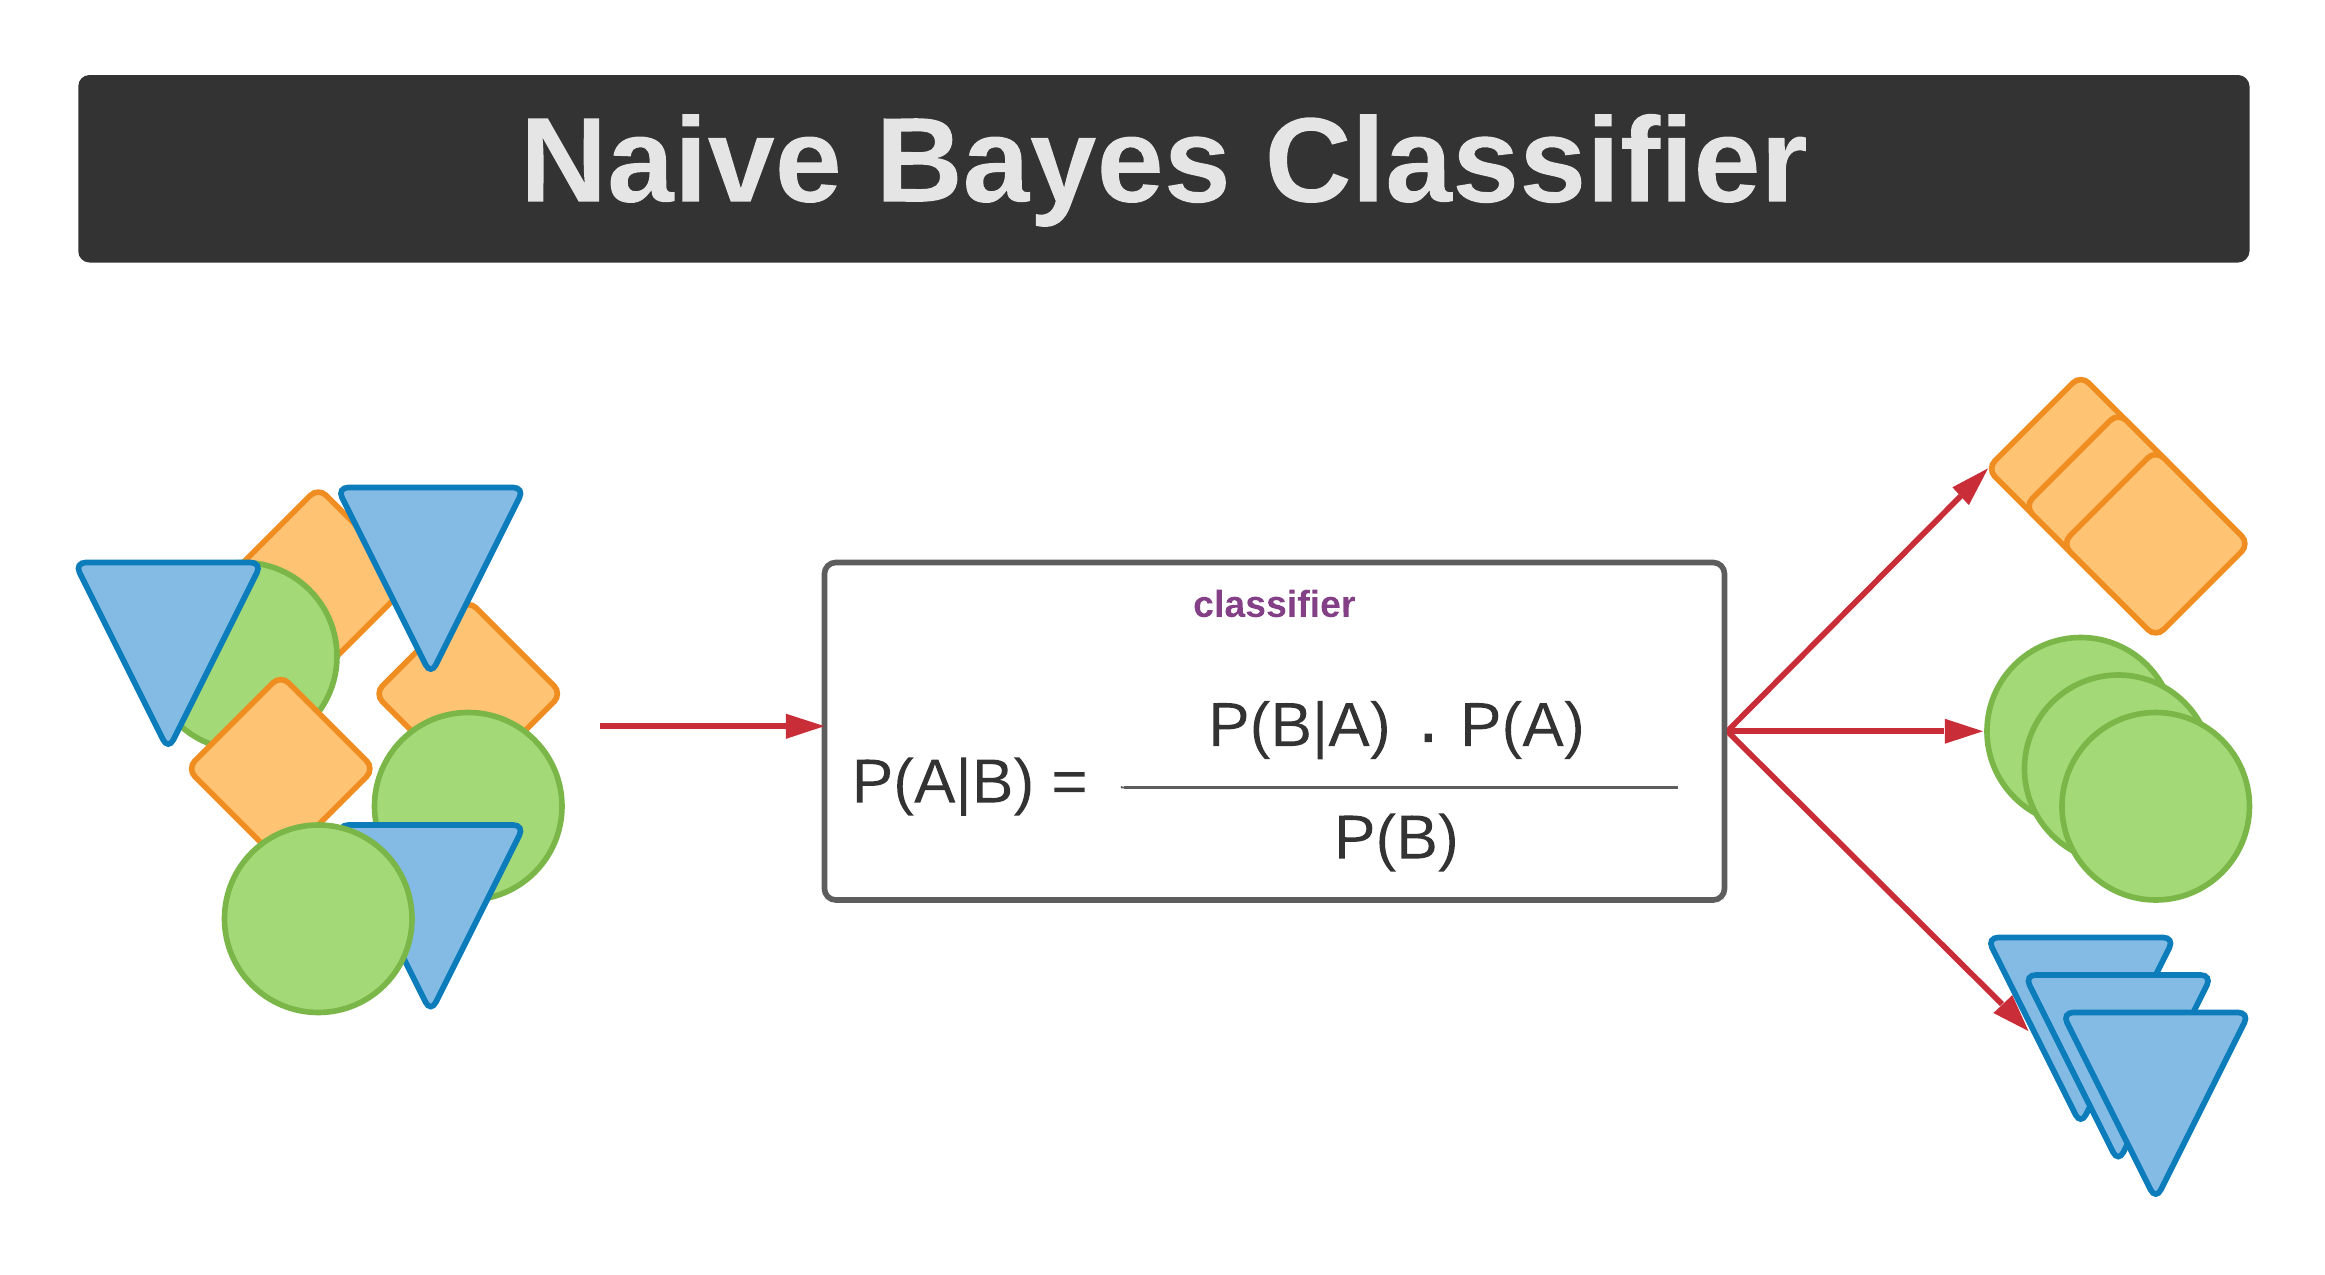
\includegraphics[scale=0.4]{notebooks/ML/img/naive_bayes_diagram.png}
    \caption{Naive Bayes Diagram}
\end{figure}

La formulación es la siguiente: 
$$
P(y | x^1 , \dots , x^M) = \frac{P(y)P(x^1 , \dots , x^M| y)}{P(x^1 , \dots , x^M)} = \frac{P(y)\prod_{j=1}^M P(x^j | y)}{P(x^1 , \dots , x^M)} \propto P(y)\prod_{j=1}^M  P(x^j | y)
$$
y la predicción se realiza según 
$$
\hat{y} = \text{argmax}_{y} P(y)\prod_{j=1}^M  P(x^j | y)
$$

\subsection{Gaussian Naive Bayes}

Aquí consideramos que $x^{j} | y \sim \mathcal{N}(\mu_j , \sigma_j^2)$ , es decir, cada feature sigue una distribución normal según:
$$
P(x^j | y) = \frac{1}{\sqrt{2\pi\sigma_j^2}}\exp \left(- \frac{(x^j - \mu_j)^2}{2\sigma_j^2} \right )
$$
donde la media y varianza $\mu_j$ y $\sigma_j$ respectivamente, son calculados a través de la máxima verosimilitud, es decir, si $x_{i} = (x^{1}_i, x^{2}_i, \dots x^{M}_i)$ con $i \in \{1, \dots, N\}$ los datos, entonces
$ \mu_{j} = \frac{1}{N}\sum_{i=1}^{N}x_{i}^{j}$ y $ \sigma_{j} = \frac{1}{N-1}\sum_{i=1}^{N}(x_{i}^{j}-\mu_{j})^2$. Notar que esto se debe calcular utilizando los datos de la clase respectiva $y$. 

La definición anterior funciona bien con tipos de data numéricos. 

\begin{figure}[H]
    \center
    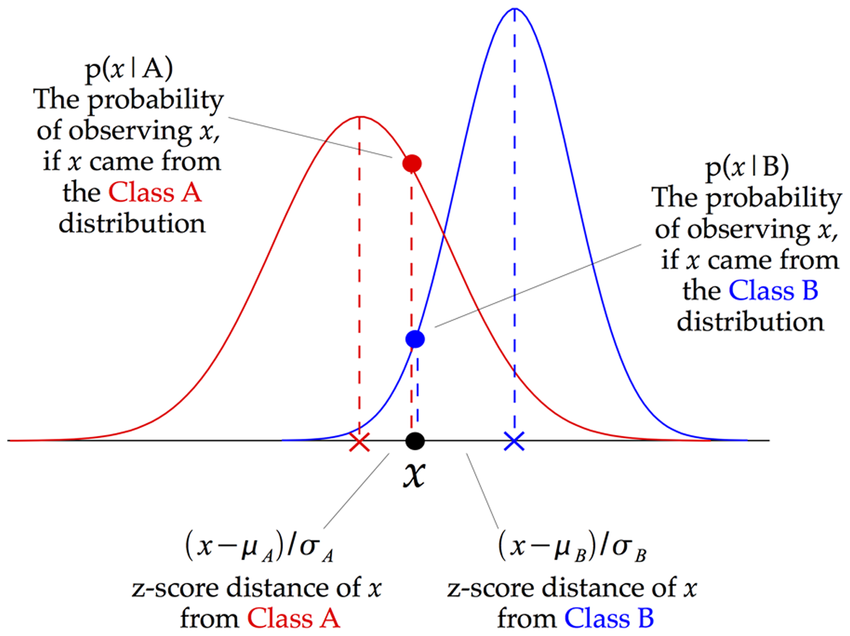
\includegraphics[scale=2]{notebooks/ML/img/gaussian_naive_bayes_diagram.png}
    \caption{Gaussian Naive Bayes Diagram}
\end{figure}

\subsection{Multinomial Naive Bayes}

Aquí consideramos que $x^j | y$ sigue una distribución multinomial donde los parámetros $(p_{j_1}, \dots , p_{j_k})$ de esta distribución son calculados según 
$$
p_{j_k} = \frac{N_{j_k} + \alpha}{N_j + \alpha}  
$$

Donde $N_{j_k}$ es la cantidad de veces que la categoría $k$ de la feature $j$ aparece en los datos con clase $y$ del conjunto de entrenamiento y $N_j = \sum_k N_{j_k}$. El parámetro $\alpha$ es un \textit{Smoothing Prior} para estabilidad numérica. 

La definición anterior funciona bien con tipos de datos categóricos. 

\section{Support Vector Machines}

Las \textit{Support Vector Machines} o SVM, son modelos de aprendizaje \textbf{supervisados} que pueden ser usados para problemas de clasificación y regresión. Se construyen a partir de la búsqueda de un hiper-plano separador y vectores de soporte que maximizan la distancia entre las clases. 

\begin{figure}[H]
    \center
    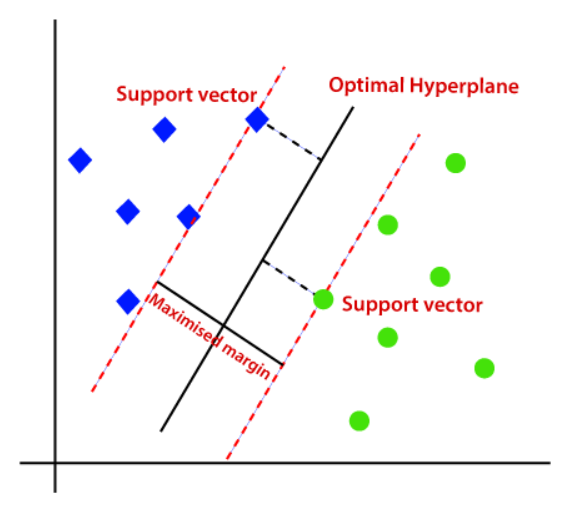
\includegraphics[scale=0.3]{notebooks/ML/img/svm_diagram.png}
    \caption{SVM Diagram}
\end{figure}

Consideremos el caso binario donde $Y \in \{0,1\}^n$ El hiper-plano separador está definido por 
$$ H = \{ x \in \mathbb{R}^n | w^{\top}x + b = 0 \} $$ 
Donde $w$ es el vector perpendicular al hiper-plano y $b$ un offset. 
De esta forma si $w^{\top}x + b > 0$ quiere decir que $x$ pertenece a la clase 1 y $w^{\top}x + b < 0$ que $x$ pertenece a la clase 0, escrito de otra forma 
$$y_i(w^{\top}x+b) \geq 1 \quad \forall i \in \{ 1 , \dots , N \}$$
En el caso de un problema de clasificación linealmente separable, existen infinitos hiper-planos que satisfacen las condiciones anteriores (basta con rotar ligeramente el hiper-plano) por lo que vamos a exigir además las siguientes condiciones sobre vectores de soporte $x_{-}$ y $x_{+}$. 

\begin{equation*}
\begin{split}
w^{\top}x_{+} + b = 1 \\
w^{\top}x_{-} + b = -1
\end{split}
\end{equation*} 

Notar entonces que con esta condición, es posible calcular el ancho $m$ de la separación entre el hiper-plano y el vector de soporte. Recordemos que la distancia $m$ de un vector $x$ a un hiperplano con vector normal $w$ viene dada por 
$$m = \frac{|\langle w, x \rangle|}{||w||}$$
Considerando la definición de los vectores de soporte, se tiene que 
$$2m = \frac{|\langle w, x_{+} \rangle|}{||w||} + \frac{|\langle w, x_{-} \rangle|}{||w||} = \frac{|1-b|}{||w||} + \frac{|-1-b|}{||w||}$$
Además el offset $b \in [0,1]$ por la definición anterior, así 
$$m = \frac{1}{||w||}$$
Finalmente, el problema de optimización quedaría de la siguiente forma 
\begin{equation*}
\begin{aligned}
\max_{\omega , b} \quad \frac{1}{||w||} \\
\textrm{s.t.} \quad y_i(w^{\top}x_i + b ) \geq 1 , \forall i \in \{ 1 , \dots N \}
\end{aligned}
\end{equation*}
Equivalente a 
\begin{equation*}
\begin{aligned}
\min_{\omega , b} \quad \frac{1}{2}||w||^2 \\
\textrm{s.t.} \quad y_i(w^{\top}x_i + b ) \geq 1 , \forall i \in \{ 1 , \dots N \}
\end{aligned}
\end{equation*}
Este problema se resuelve utilizando el \textbf{dual} (\textit{quadratic programming}) y es fundamental para la extensión no-lineal de la SVM (\textit{Kernel Trick}). 

\subsection{Soft Margin}

Los datos son usualmente no linealmente separables, por lo que hay que permitir un error en la clasificación de ciertos puntos (\textit{soft margin}). Este cambio en el problema de optimización se reduce a la siguiente regularización:

\begin{equation*}
\begin{aligned}
\min_{\omega , b} \quad \frac{1}{2}||w||^2 + C \sum_{i=1}^N \xi_i  \\
\textrm{s.t.} \quad y_i(w^{\top}x_i + b ) \geq 1  - \xi_i, \forall i \in \{ 1 , \dots N \} \hspace{0.1cm} ,\hspace{0.1cm} \xi_i \geq 0
\end{aligned}
\end{equation*}

\subsection{Kernel Trick}

En la formulación del problema dual, la función objetivo requiere el cómputo del producto interno entre todos los puntos del conjunto de entrenamiento. Si buscamos proyectar nuestra data a una dimensión mayor (aplicar algún mapeo $\phi$ para hacer la separación posible), esto se puede realizar calculando los productos $ \langle \phi(x_i) , \phi(x_j) \rangle $ para todo $i$ y $j$.

\begin{figure}[H]
    \center
    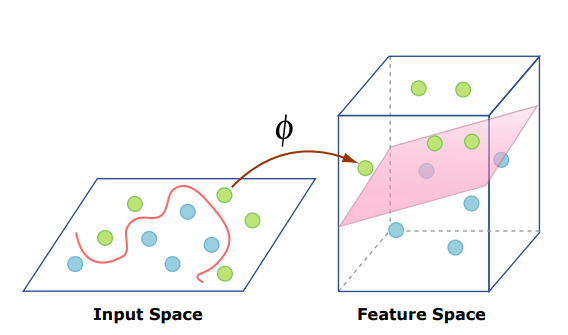
\includegraphics[scale=0.5]{notebooks/ML/img/kernel_trick.png}
    \caption{Kernel Trick}
\end{figure}

El paso fundamental del truco del kernel es que no es necesario conocer el mapeo $\phi$ explícitamente pues por el teorema de \textit{Mercer}
$$
K(x_i , x_j) = \langle \phi(x_i) , \phi(x_j) \rangle
$$
donde $K: X \times X \rightarrow \mathbb{R} $ es un kernel de \textit{Mercer} en un espacio de \textit{Hilbert} (posiblemente de dimensión infinita), por lo que solo basta que definamos $K$ para tener un posible mapeo de las características. 

\subsection{Kernels}

Para que un kernel pueda utilizarse en el contexto de las SVM, es importante que cumpla con las condiciones de \textit{Mercer}: 
\begin{itemize}
    \item Symmetry: $K(x,y) = K(y,x) \quad \forall x,y$ 
    \item Positive Semi-Definiteness: Para cualquier vector $c \in \mathbb{R}^n$, y $x_1 , \dots x_n$ una cantidad finita de puntos, se debe satisfacer que  
    $$\sum_{ij}c_ix_jK(x_i,x_j) \geq 0$$
\end{itemize}

Algunos ejemplos de \textit{kernels} que se pueden utilizar son: 

\begin{enumerate}
    \item \textbf{Linear Kernel}: $K(x,y) = \langle x , y \rangle$. 
    
    El más útil cuando la data es linealmente separable. 
    \item \textbf{Polynomial Kernel}: $K(x,y) = (x^{\top}y + c)^d$. 
    
    El parámetro $d$ controla el nivel de complejidad del kernel pero valores muy altos podrían llevar a overfitting.
    \item \textbf{Gaussian Radial Basis Function (RBF) Kernel}: $K(x,y) = e^{-\gamma||x-y||^2}$. 
    
    Este kernel es el más popular pues \textbf{mapea los datos a un espacio de dimensión infinita}. El parámetro $\gamma$ controla la complejidad de los \textit{decision boundaries} al agregar mayor o menor spread al kernel. 
    \item \textbf{Sigmoid Kernel}: $K(x,y) = \text{tanh}(ax^{\top}y + b)$
\end{enumerate}

\begin{figure}[H]
    \center
    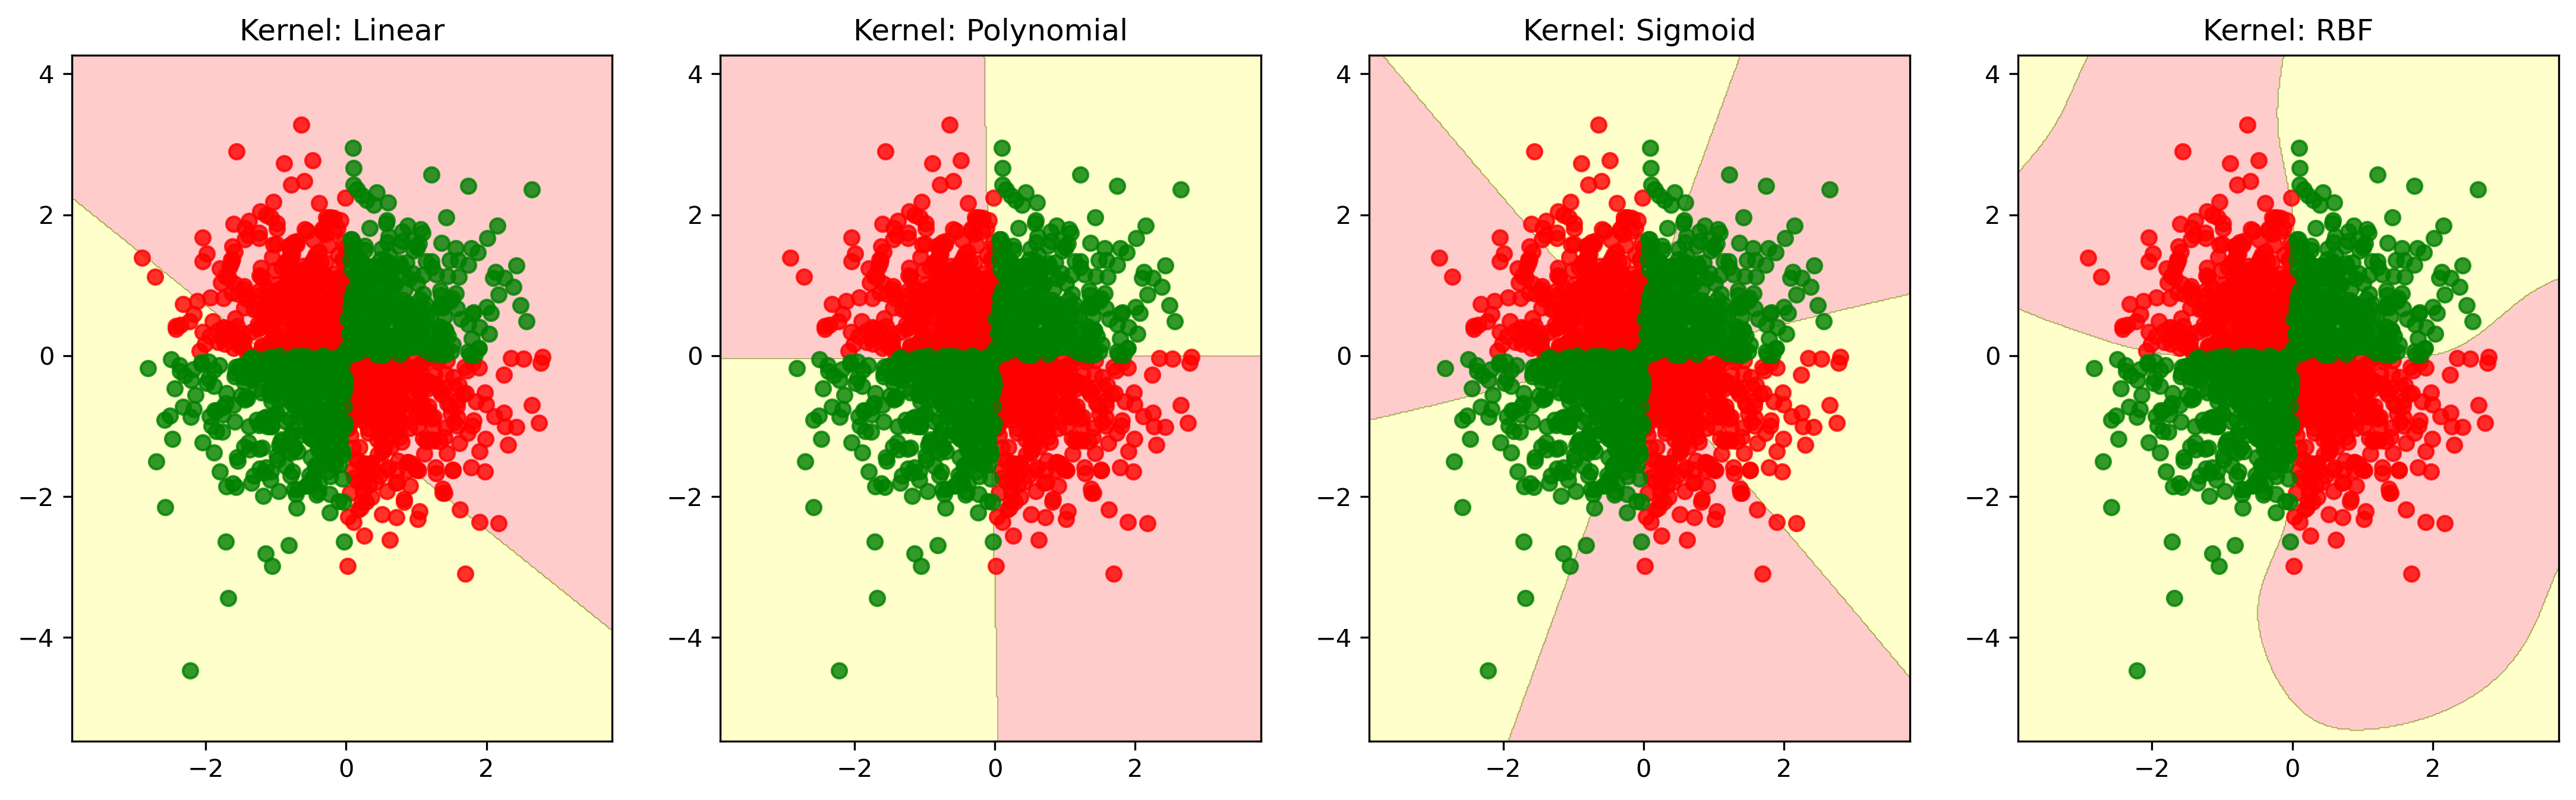
\includegraphics[scale=0.35]{notebooks/ML/img/kernel_decision_boundaries.png}
    \caption{Kernel Decision Boundaries}
\end{figure}

\section{ARIMA}

ARIMA es la abreviación de \textit{Auto-Regressive Integrated Moving Average} y es un método estadístico para realizar forecasting sobre series de tiempo que integra los siguientes conceptos:

\begin{enumerate}
    \item Toma en consideración patrones de crecimiento/decrecimiento en la serie de tiempo (\textit{Auto-Regressive}). 
    \item Estima tasa de crecimiento/decrecimiento (\textit{Integrated}).
    \item Controla el ruido entre datos consecutivos en el tiempo (\textit{Moving Average}).
\end{enumerate}

La fórmula general para este tipo de modelos viene dada por 
$$
Y_t = c + \phi_1y^d_{t-1} + \dots + \phi_py^d_{t-p} + \theta_1e_{t-1} + \dots + \theta_q e_{t-q} + e_t
$$
Aquí $c$ es una constante y $e$ es un término de error. Los modelos de este tipo son escritos como ARIMA($p,d,q$) donde: 

\begin{itemize}
    \item $p$ es la cantidad de tiempos en que la variable es mirada al pasado (Lag).
    \item $d$ es la cantidad de veces que la variable es diferenciada para producir una señal estacionaria. $d=0$ refiere a que la señal ya es estacionaria, $d=1$ es que la señal crece/decrece linealmente y $d=2$ es que la señal crece exponencialmente. 
    \item $q$ representa la cantidad de lag para el término de error $e$, esto captura el \textit{Moving Average}.
\end{itemize}

\subsection{P Value}

En la práctica, es posible determinar el valor de $p$ a través del \textit{Partial Autocorrelation Plot}. Este gráfico muestra la relación de un valor en la serie de tiempo con \textbf{un solo lag} (eliminando relaciones de tiempos intermedios ajustando una regresión lineal y quedándose sólo con el parámetro correspondiente).
\begin{figure}[H]
    \center
    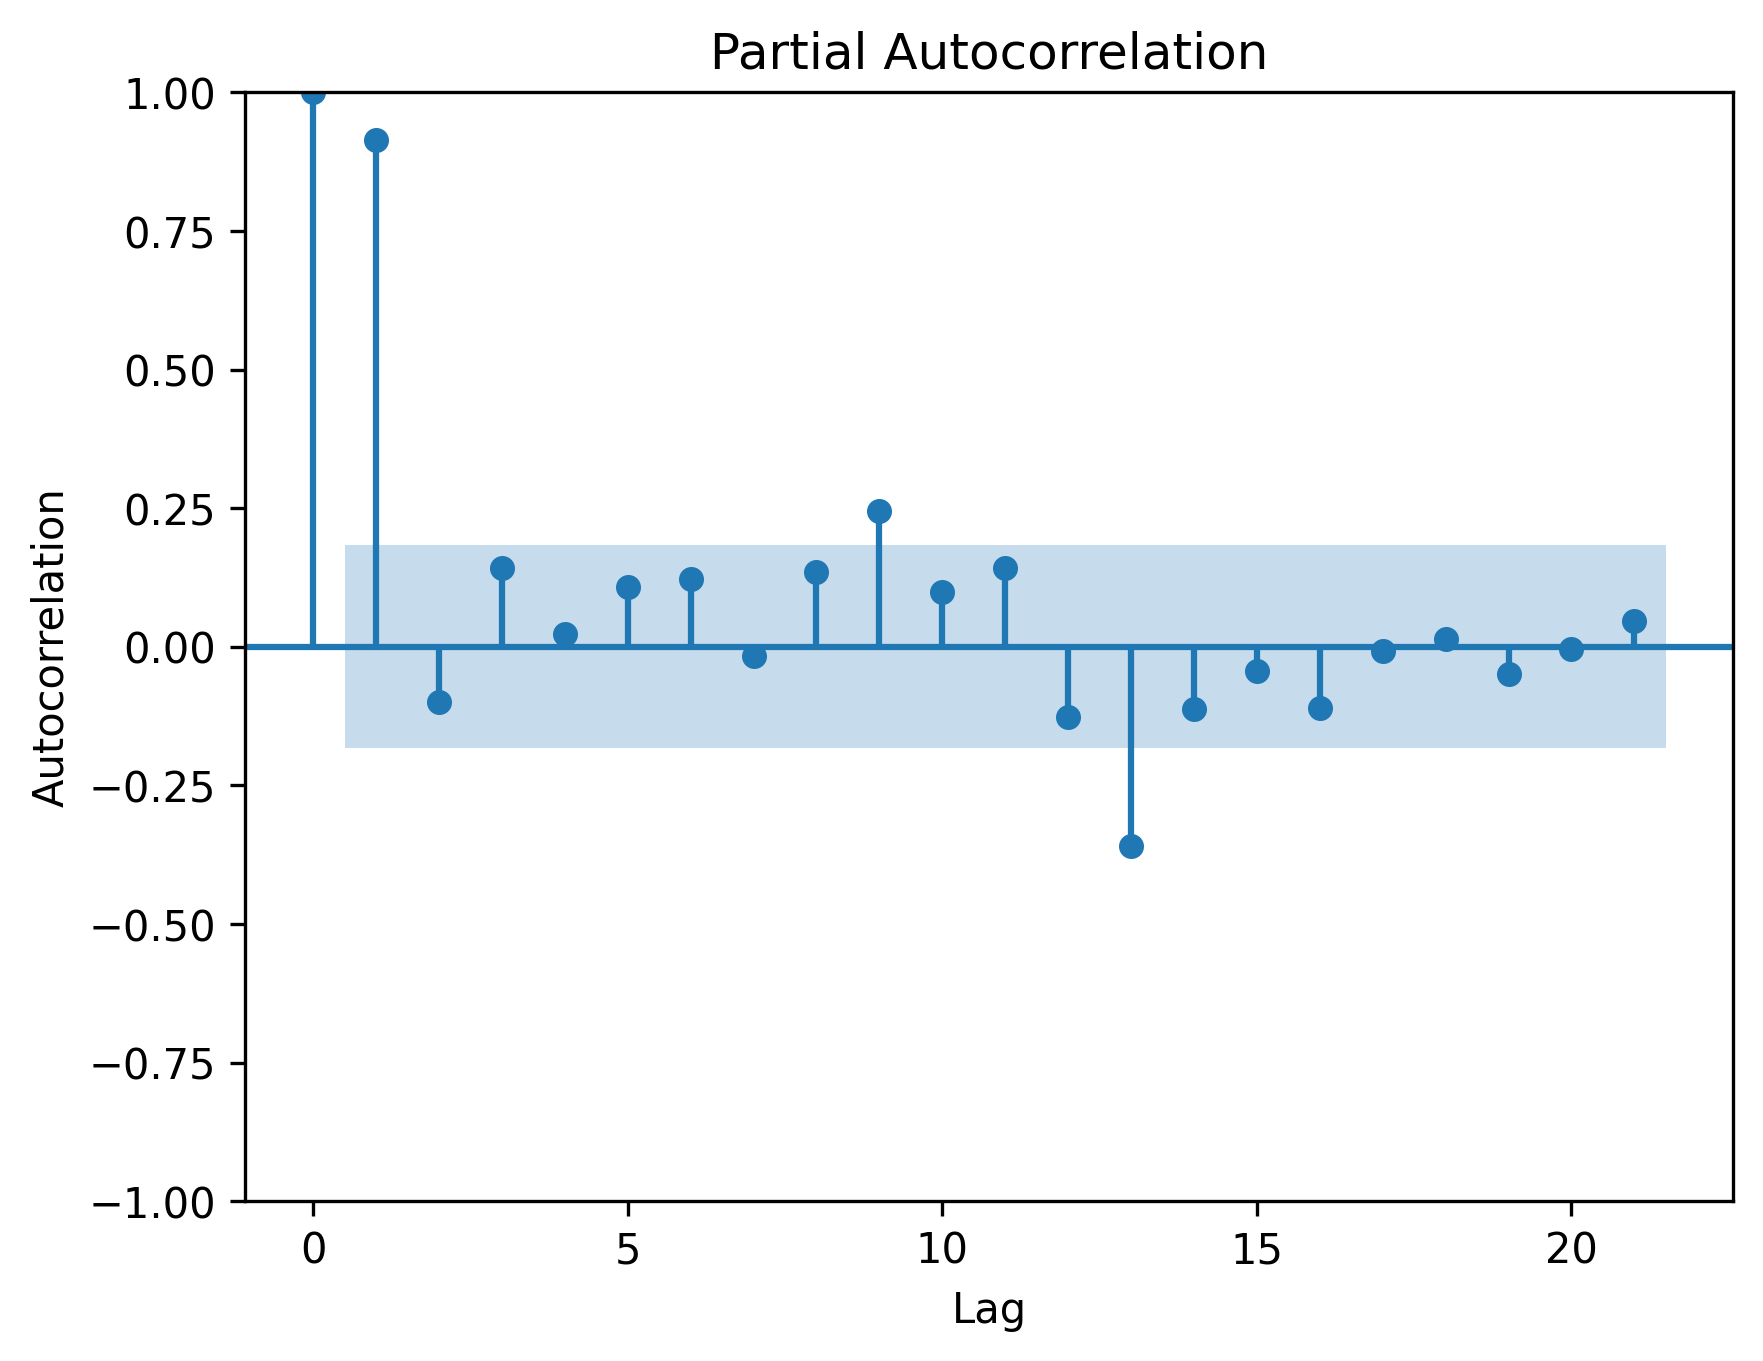
\includegraphics[scale=0.5]{notebooks/ML/img/partial_autocorrelation.png}
    \caption{Partial Autocorrelation Plot}
\end{figure}
El valor óptimo es el último punto después del cual todos los lags están dentro de las bandas azules (intervalos de confianza), en este caso $p=13$. 

\subsection{D Value}

El valor de $d$ se puede calcular diferenciando la serie de tiempo hasta encontrar una serie estacionaria. Esto lo podemos medir con un test estadístico de estacionalidad (\textit{Augmented Dickey Fuller Test}).

\begin{figure}[H]
    \center
    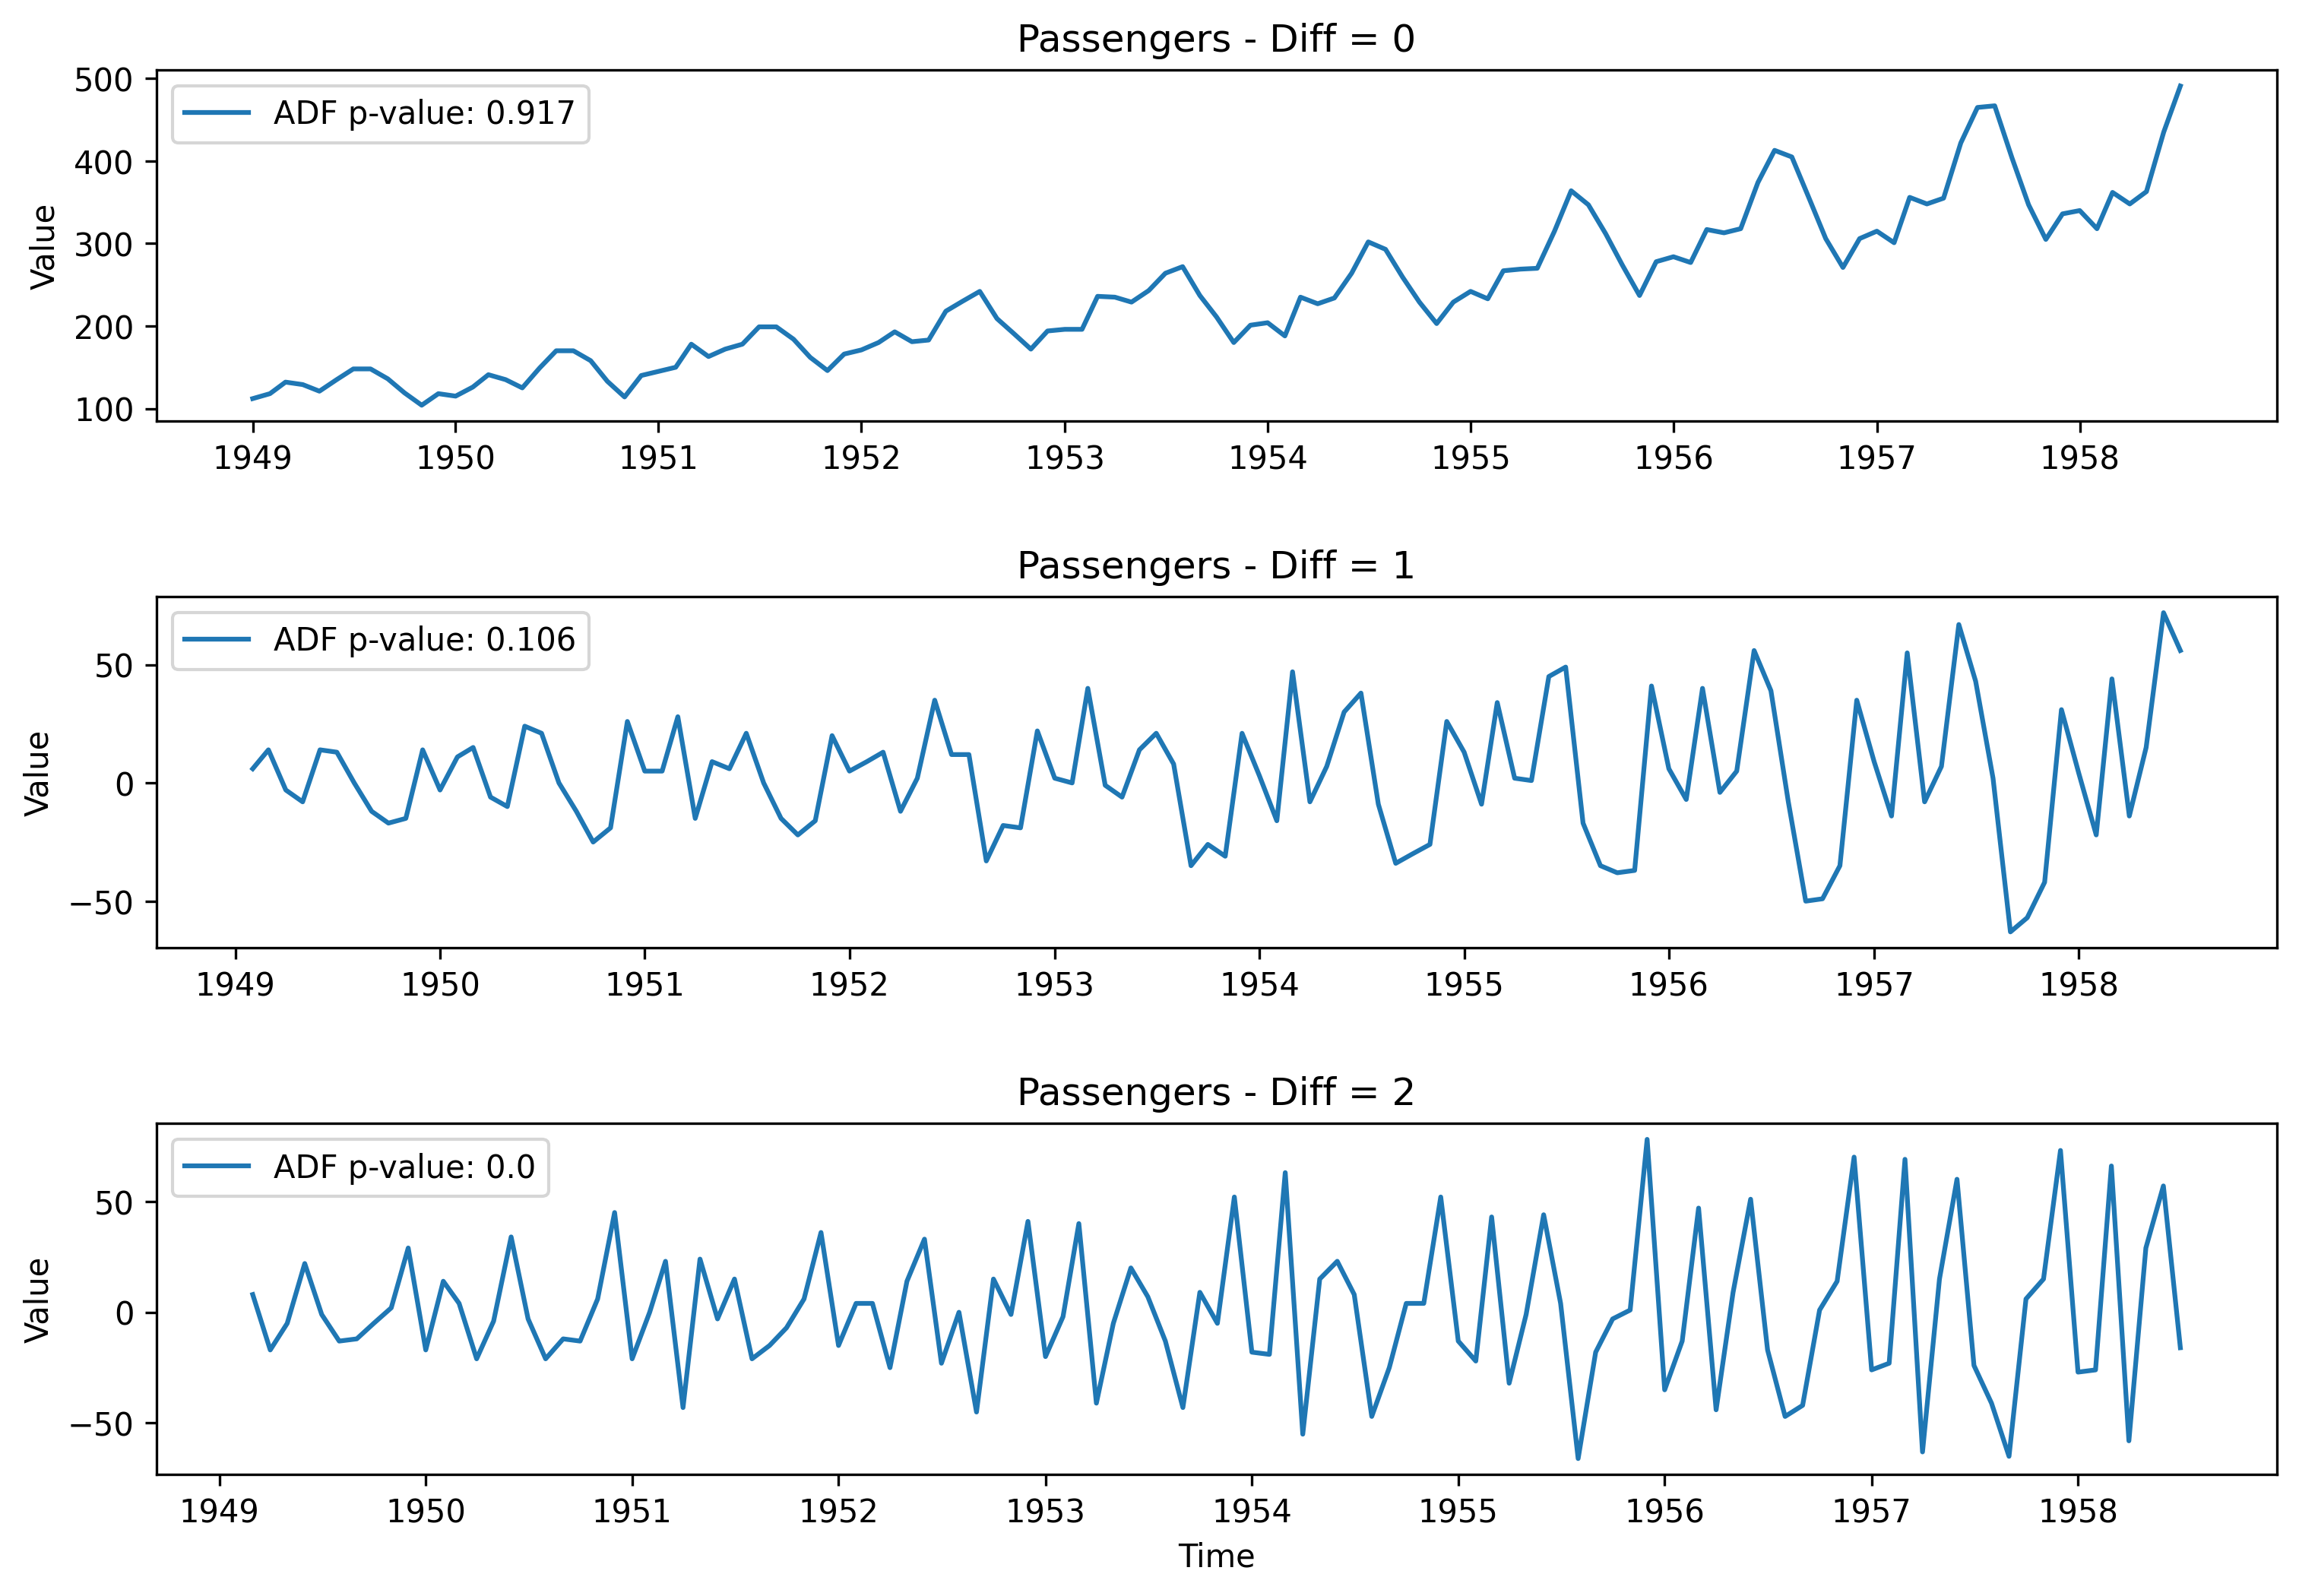
\includegraphics[scale=0.5]{notebooks/ML/img/time_series_differentiation.png}
    \caption{Time Series Differentiation Plot}
\end{figure}

Vemos que el $p$-valor en la segunda diferenciación ya es lo suficientemente pequeño para asumir estacionalidad en la serie de tiempo, así $d=2$. 

\subsection{Q Value}
Finalmente, para determinar el valor $q$ es posible ver el \textit{Autocorrelation Plot} que muestra la relación de un valor en la serie de tiempo con \textbf{todos los $p$ lags} anteriores. 
\begin{figure}[H]
    \center
    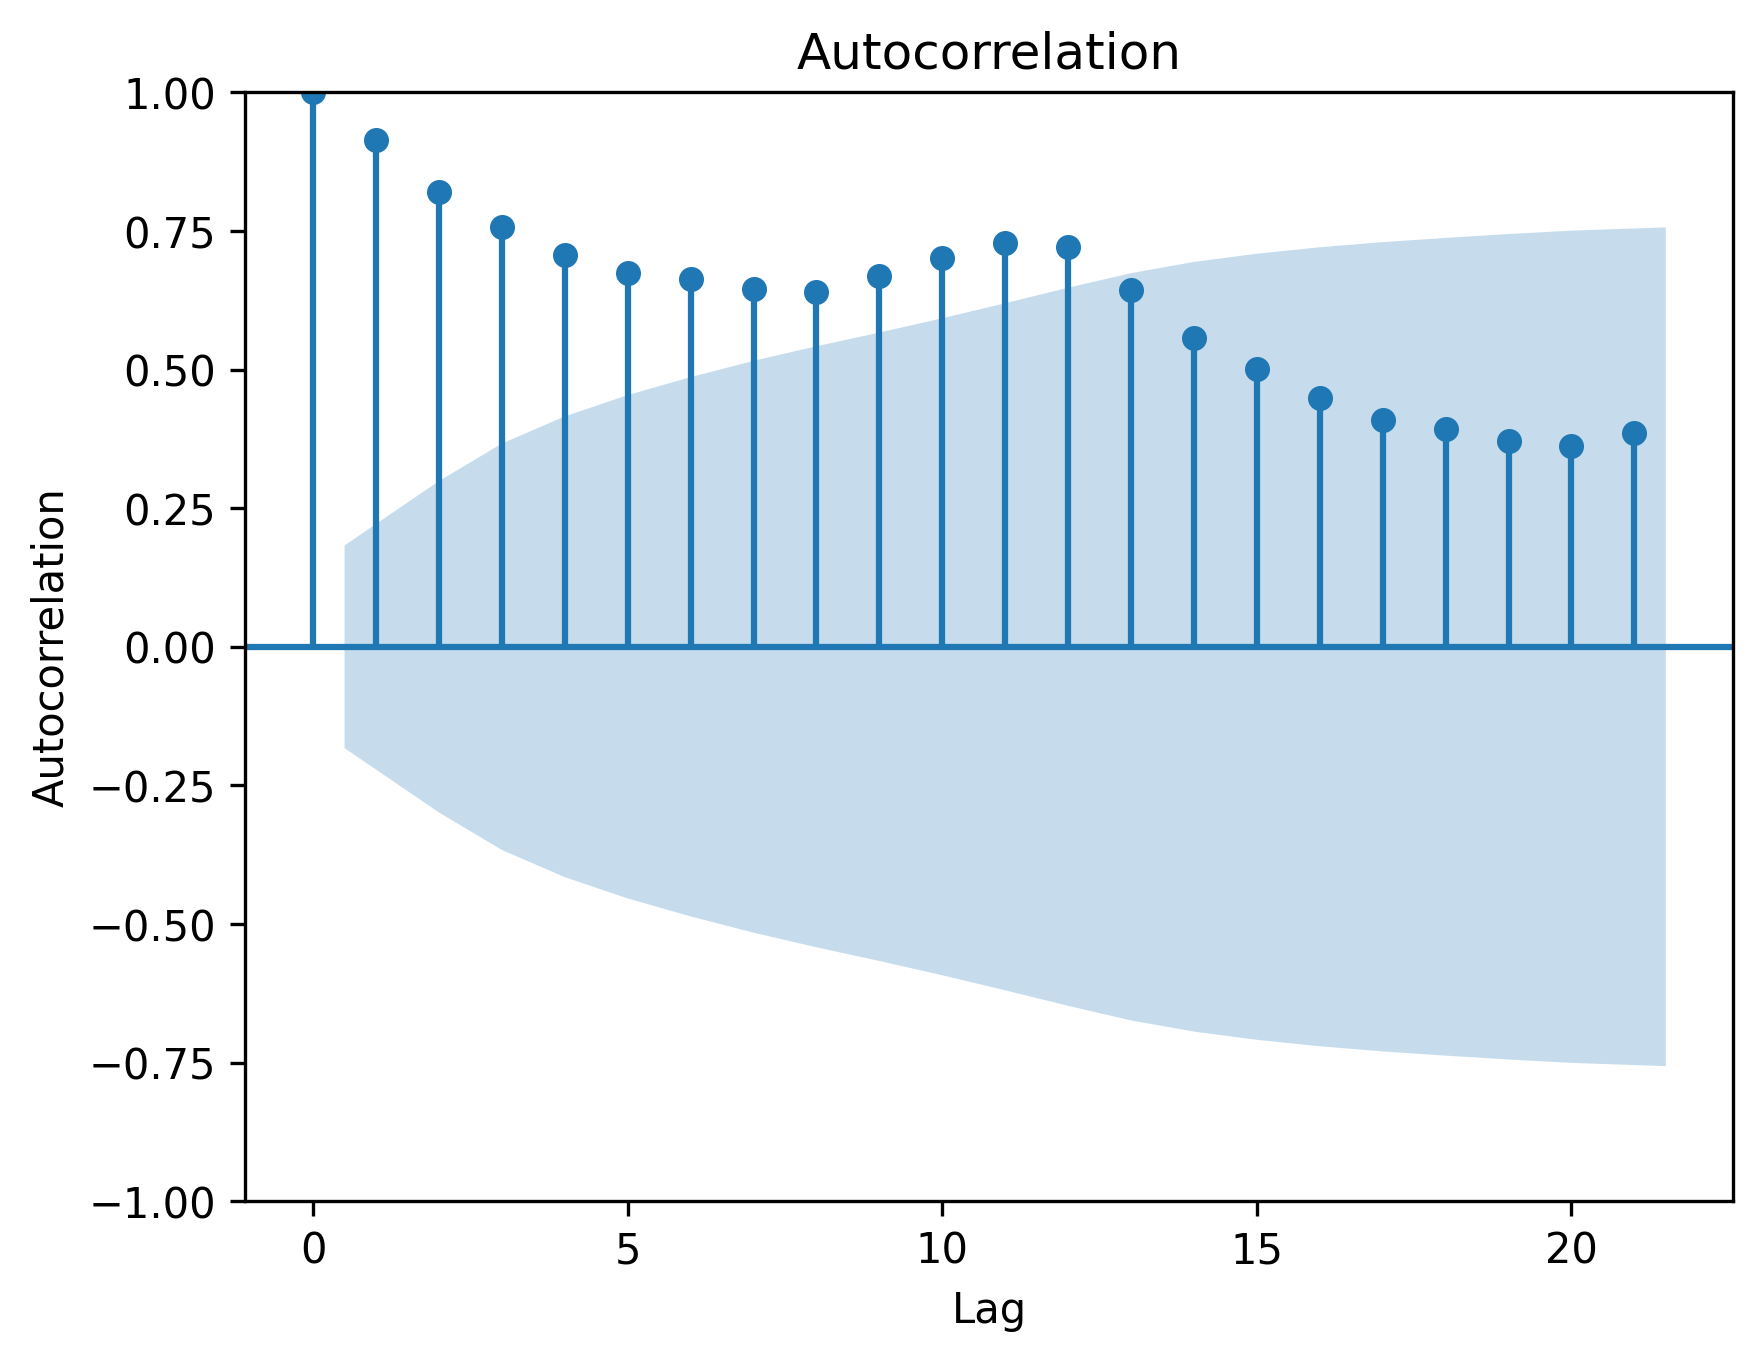
\includegraphics[scale=0.5]{notebooks/ML/img/autocorrelation.png}
    \caption{Autocorrelation Plot}
\end{figure}
En este caso, el último valor anterior a que todos los lag caigan en la zona azul, es $q=12$.
\begin{figure}[H]
    \center
    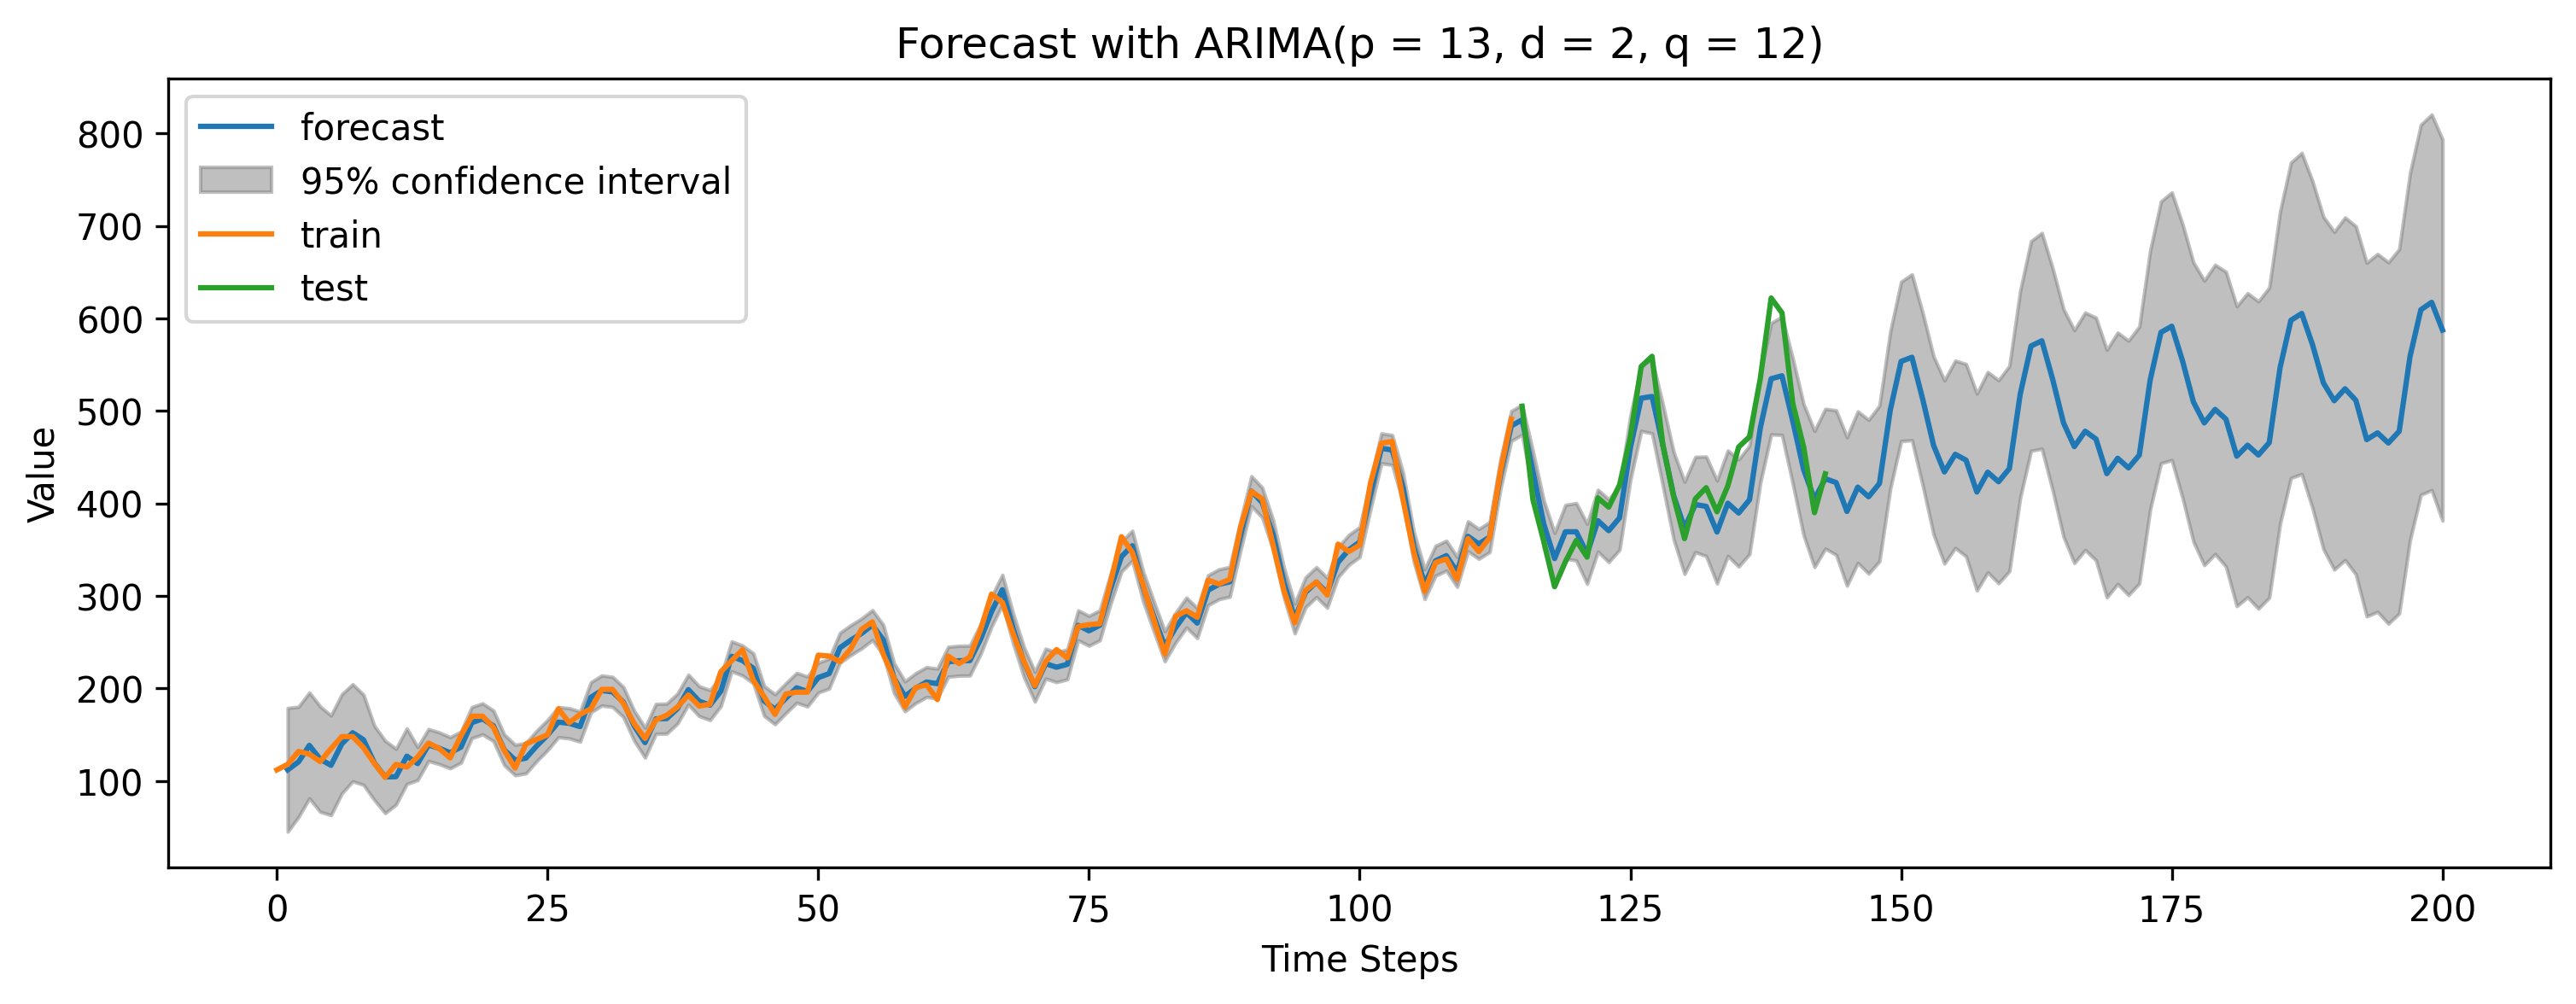
\includegraphics[scale=0.5]{notebooks/ML/img/arima_results.png}
    \caption{ARIMA over Flight Passengers Forecasting}
\end{figure}

\section{K-Means}

El algoritmo de \textit{K-Means} es un algoritmo \textbf{no supervisado de clustering}. 
El objetivo es agrupar los datos alrededor de \textbf{centroides} de tal forma en que se minimice la suma de alguna medida de distancia. Vale decir, encontrar el conjunto $ S = \{ S_1 , \dots, S_k \} $ de clusters ($k$ hiperparámetro) tal que

\begin{equation*}
\begin{aligned}
S = \argmin_{S} \sum_{i=1}^{k}\sum_{x \in S_i}||x- \mu_i||_{2}^2
\end{aligned}
\end{equation*}

Notar que $\mu_i = \frac{1}{|S_i|}\sum_{x \in S_i}x_i$ es el centroide del cluster $S_i$ para todo $i$. El algoritmo que realiza esta búsqueda es el siguiente: 
\begin{enumerate}
    \item Seleccionar $k$ centroides aleatorios del conjunto de datos. 
    \item Asignar cada punto del conjunto de datos al centroide más cercano. 
    \item Actualizar el nuevo centroide del cluster $S_i$ según $\mu_i = \frac{1}{|S_i|}\sum_{x \in S_i}x_i$. Iterar los pasos 2 y 3 hasta que la asignación no cambie.
\end{enumerate}

\begin{figure}[H]
    \center
    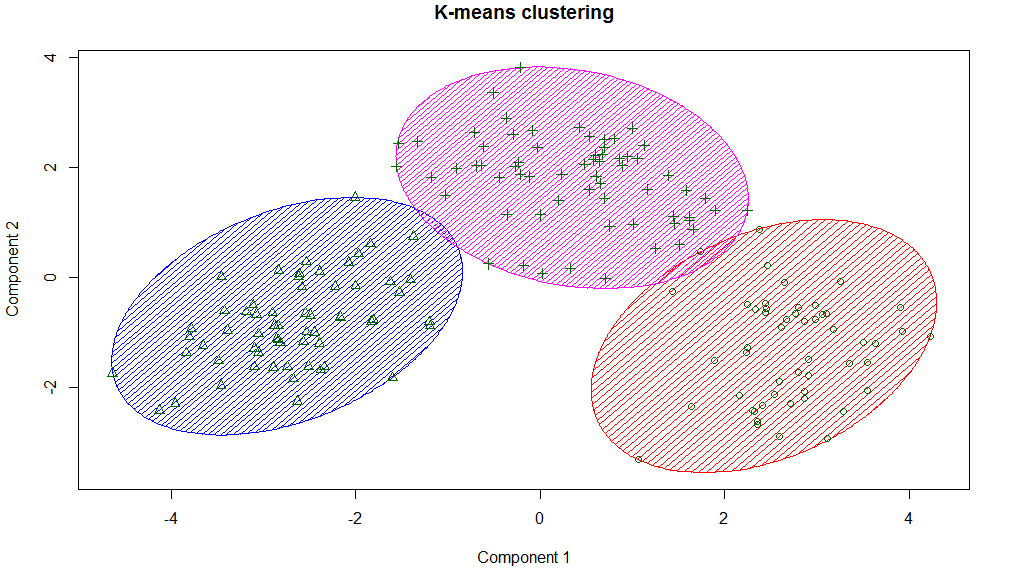
\includegraphics[scale=0.25]{notebooks/ML/img/k_means_diagram.png}
    \caption{K-Means Diagram}
\end{figure}

\textbf{Este algoritmo siempre converge pero no asegura el óptimo global}. Además, la distancia euclidiana asume que los clusters tienen \textbf{forma esférica}. Por último, es muy \textbf{sensible a outliers}

La selección del hiper-parámetro $k$ se puede hacer utilizando el método del codo (\textit{Elbow Method}). Es decir, calcular el error de la función objetivo para distintos valores de $k$ y seleccionar el menor valor de $k$ tal que la función objetivo no cambie en gran magnitud con los valores siguientes. 

\begin{figure}[H]
    \center
    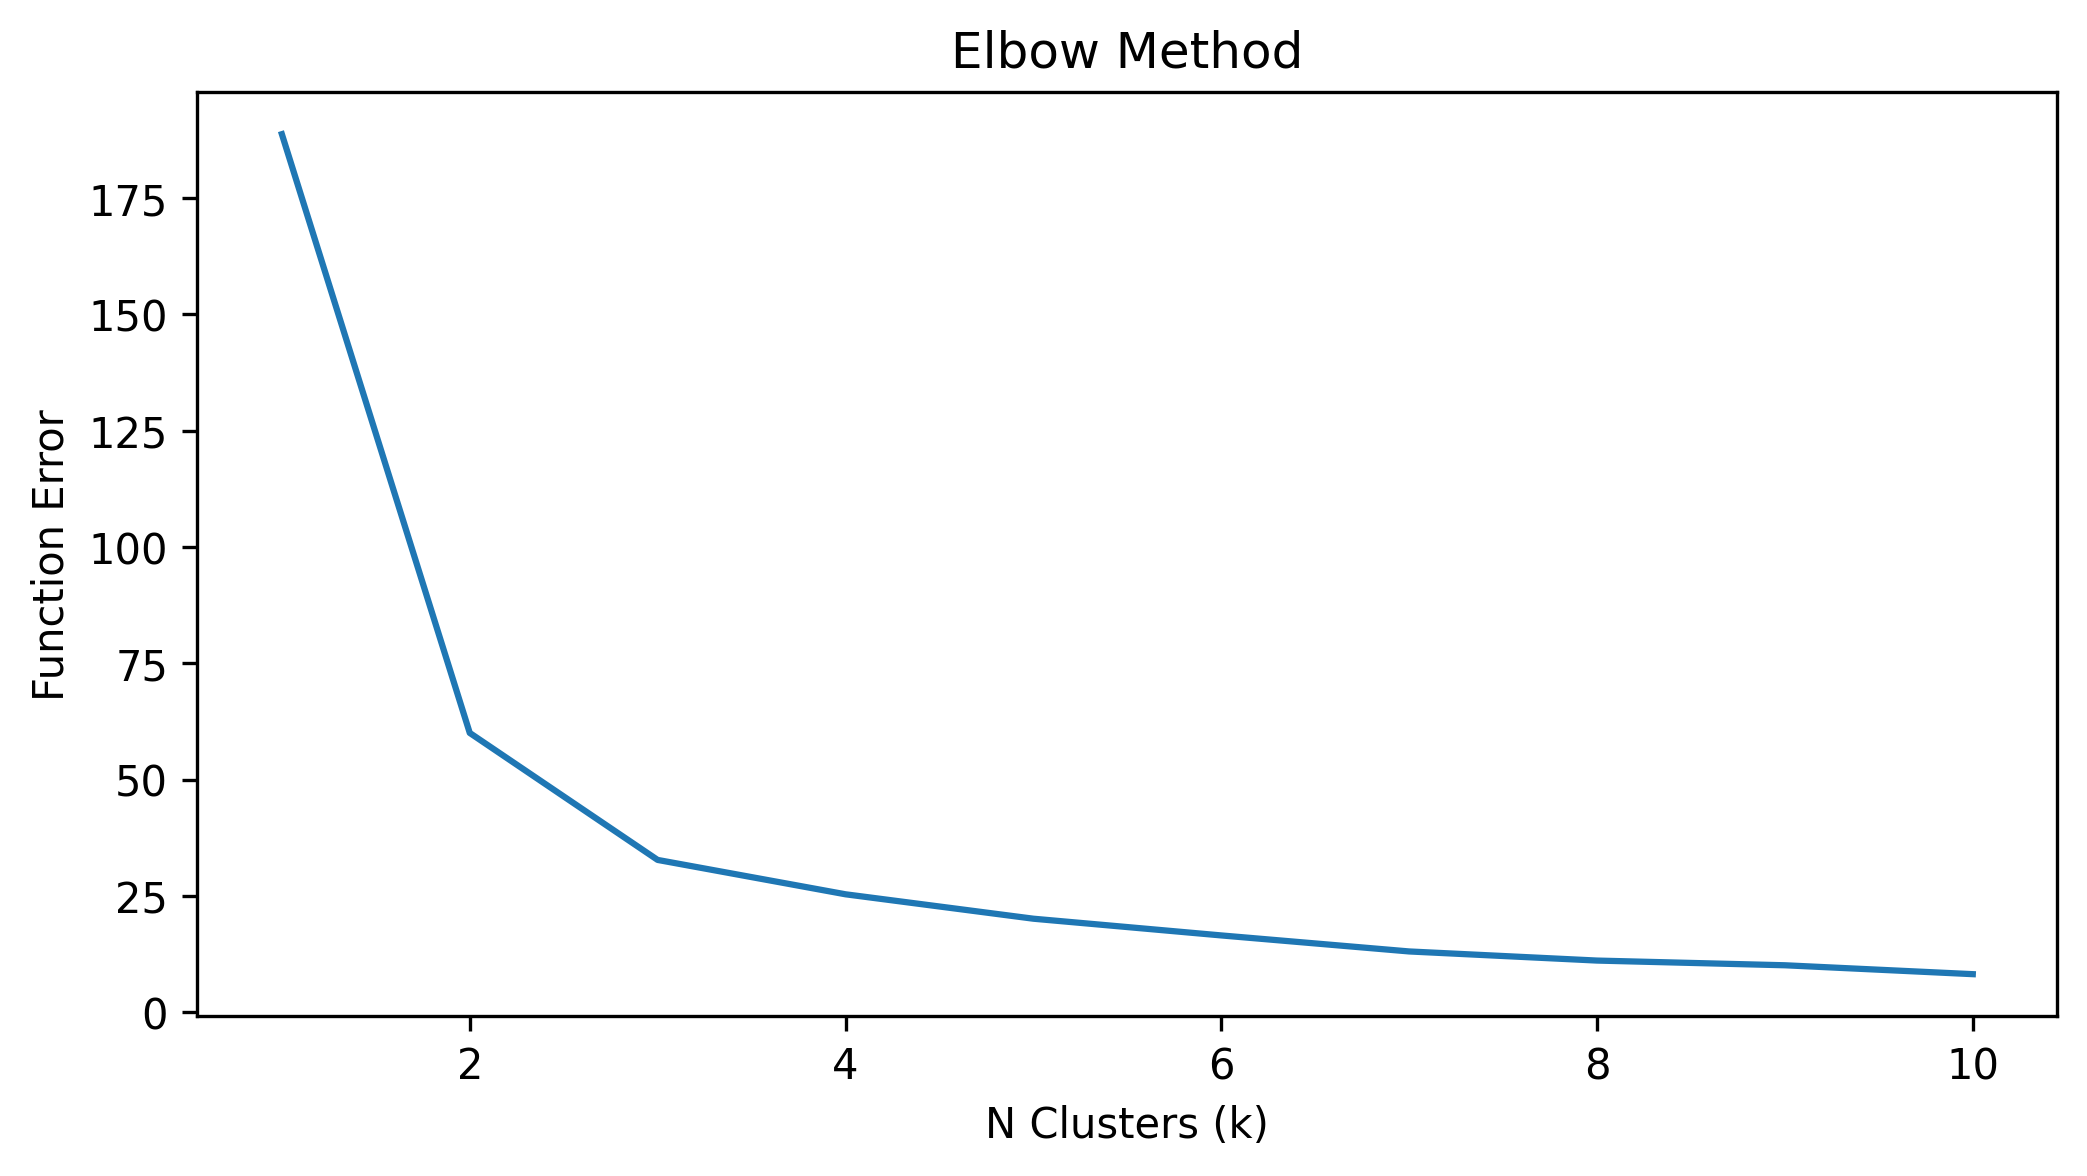
\includegraphics[scale=0.45]{notebooks/ML/img/elbow_method_k_means.png}
    \caption{Elbow Method}
\end{figure}

En este ejemplo, el valor óptimo de clusters con el \textit{Elbow Method} es $k=3$.  

\section{Hierarchical Clustering}

Los algoritmos de \textit{Hierarchical Clustering} buscan crear jerarquías de grupos conformados por elementos del dataset. Estos pueden ser de 2 categorías: 

\begin{enumerate}
    \item \textbf{Agglomerative}: Cada observación comienza en un grupo y comienzan a juntarse. 
    \item \textbf{Divisive}: Comenzar de un grupo y empezar a dividir.
\end{enumerate}

\begin{figure}[H]
    \center
    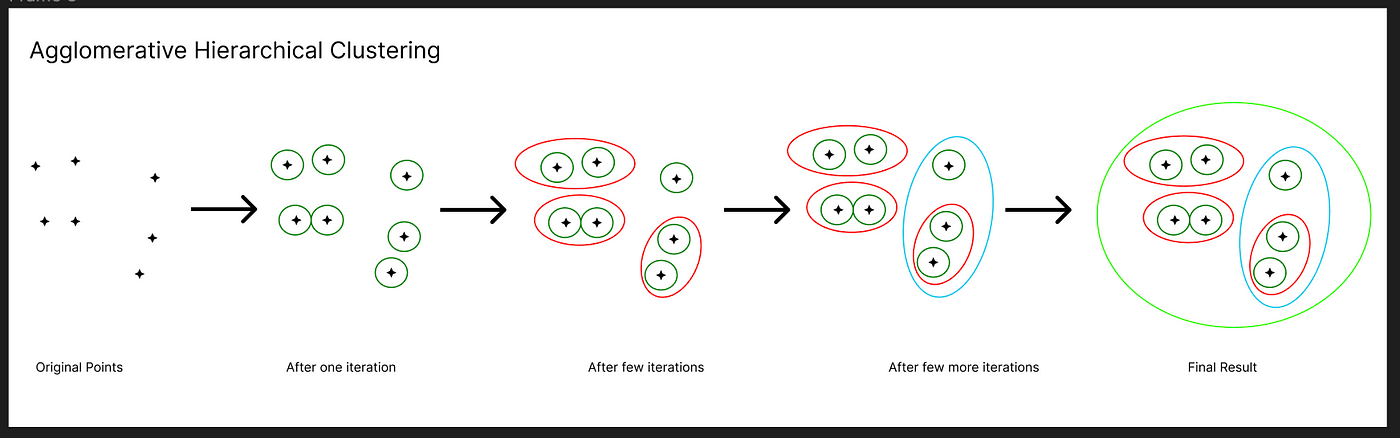
\includegraphics[scale=0.25]{notebooks/ML/img/agg_clustering.png}
    \caption{Agglomerative Clustering Example}
\end{figure}

En el caso aglomerativo, los clusters más cercanos se juntan para formar un nuevo grupo. Existen distintos criterios para definir cercanía: 

\begin{itemize}
    \item \textbf{Single}: Los elementos más cercanos entre clusters. $$\min_{a \in A, b \in B} d(a,b)$$
    \item \textbf{Complete}: Los elementos más alejados entre clusters.  $$\max_{a \in A, b \in B} d(a,b)$$
    \item \textbf{Average}: La distancia promedio entre todos los puntos de ambos clusters. $$\frac{1}{|A| \cdot |B|}\sum_{a \in A} \sum_{b \in B} d(a,b)$$
    \item \textbf{Ward}: Minimizar la varianza entre clusters luego de la unión. 
    $$\frac{|A|\cdot|B|}{|A \cup B|}||\mu_A - \mu_B||^2 = \sum_{x \in A \cup B}||x - \mu_{A \cup B}||^2 - \sum_{x \in A}||x - \mu_{A}||^2 - \sum_{x \in B}||x - \mu_{B}||^2$$
\end{itemize}

Estas divisiones se pueden visualizar a través de \textbf{Dendogramas} y cada criterio cambiará la forma de definir los clusters.

\begin{figure}[H]
    \center
    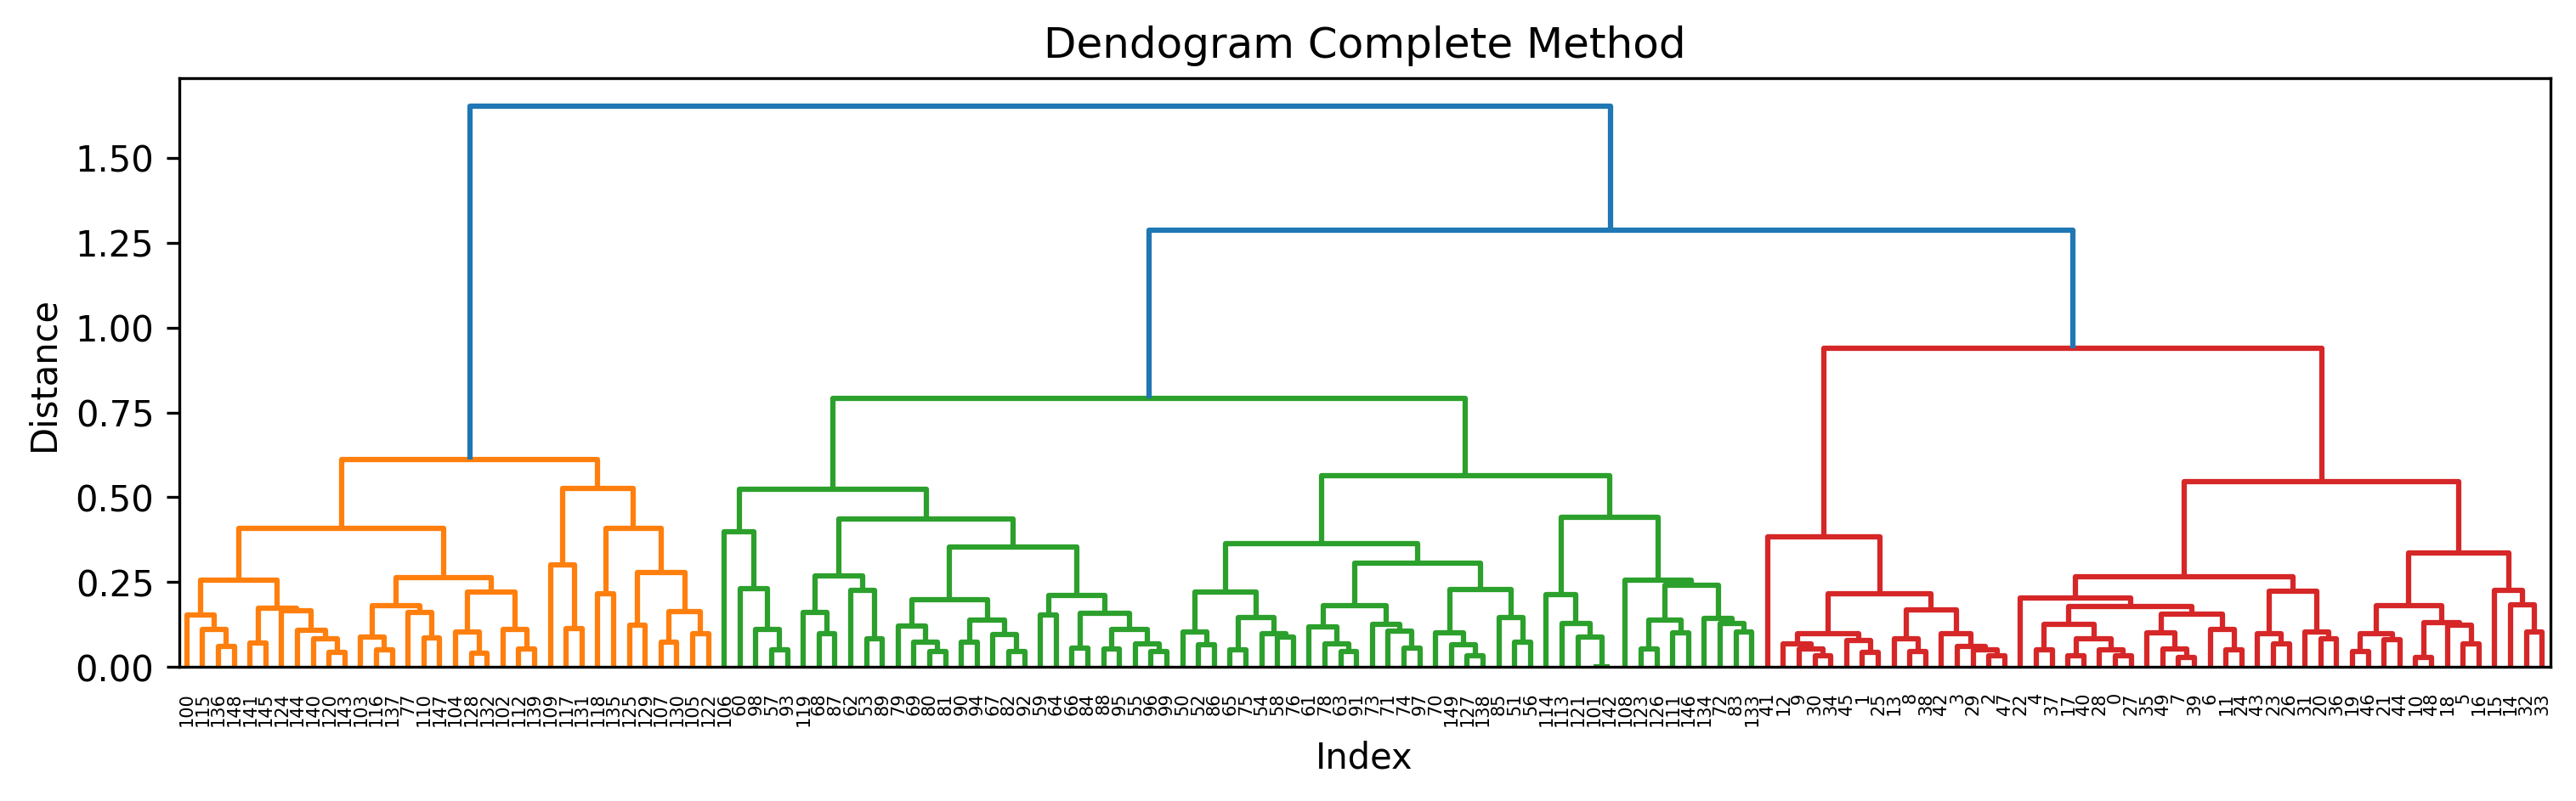
\includegraphics[scale=0.5]{notebooks/ML/img/complete_dendogram_iris.png}
    \caption{Complete Dendogram over Iris Dataset}
\end{figure}

\begin{figure}[H]
    \center
    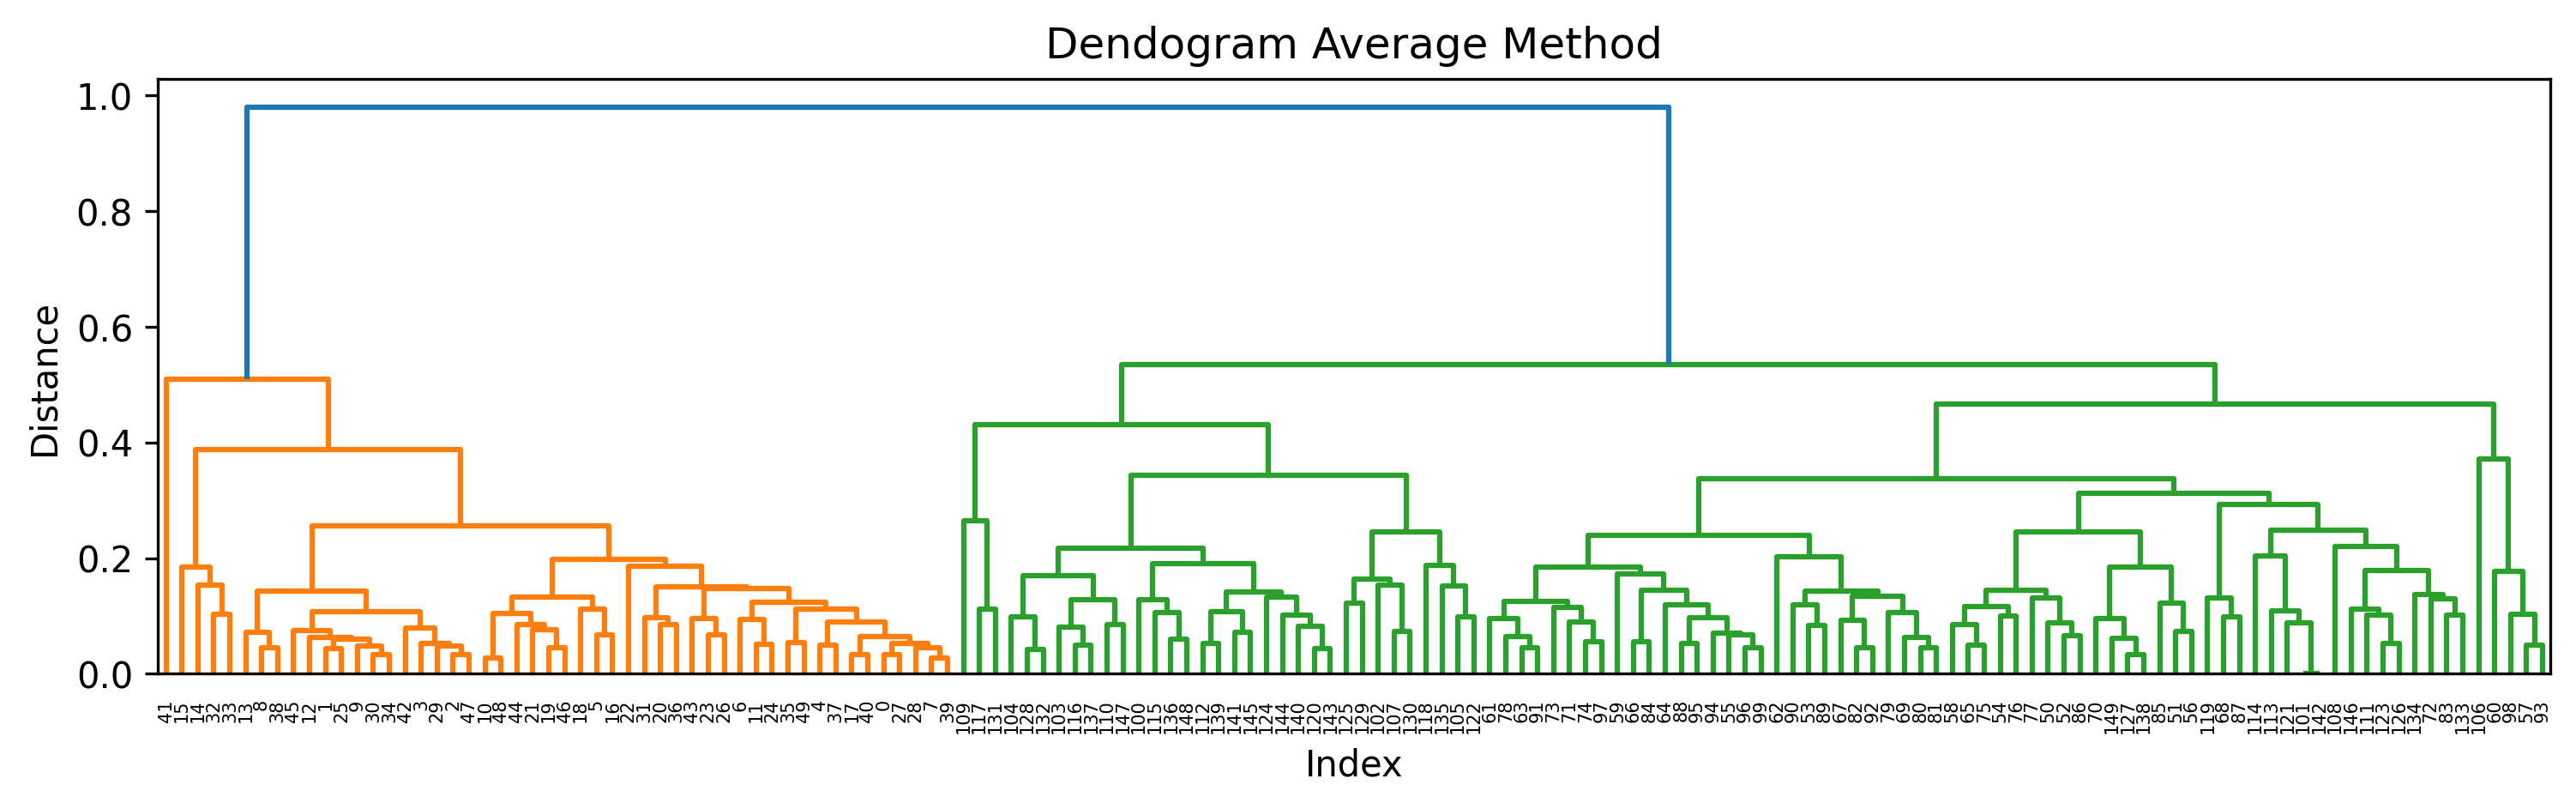
\includegraphics[scale=0.5]{notebooks/ML/img/average_dendogram_iris.png}
    \caption{Average Dendogram over Iris Dataset}
\end{figure}

\section{DBSCAN}

El algoritmo DBSCAN (\textit{Density-based spatial clustering of applications with noise}) es un algoritmo basado en densidad que permite resolver problemas de \textbf{clustering} y realizar \textbf{outlier detection}. 

\begin{figure}[H]
    \center
    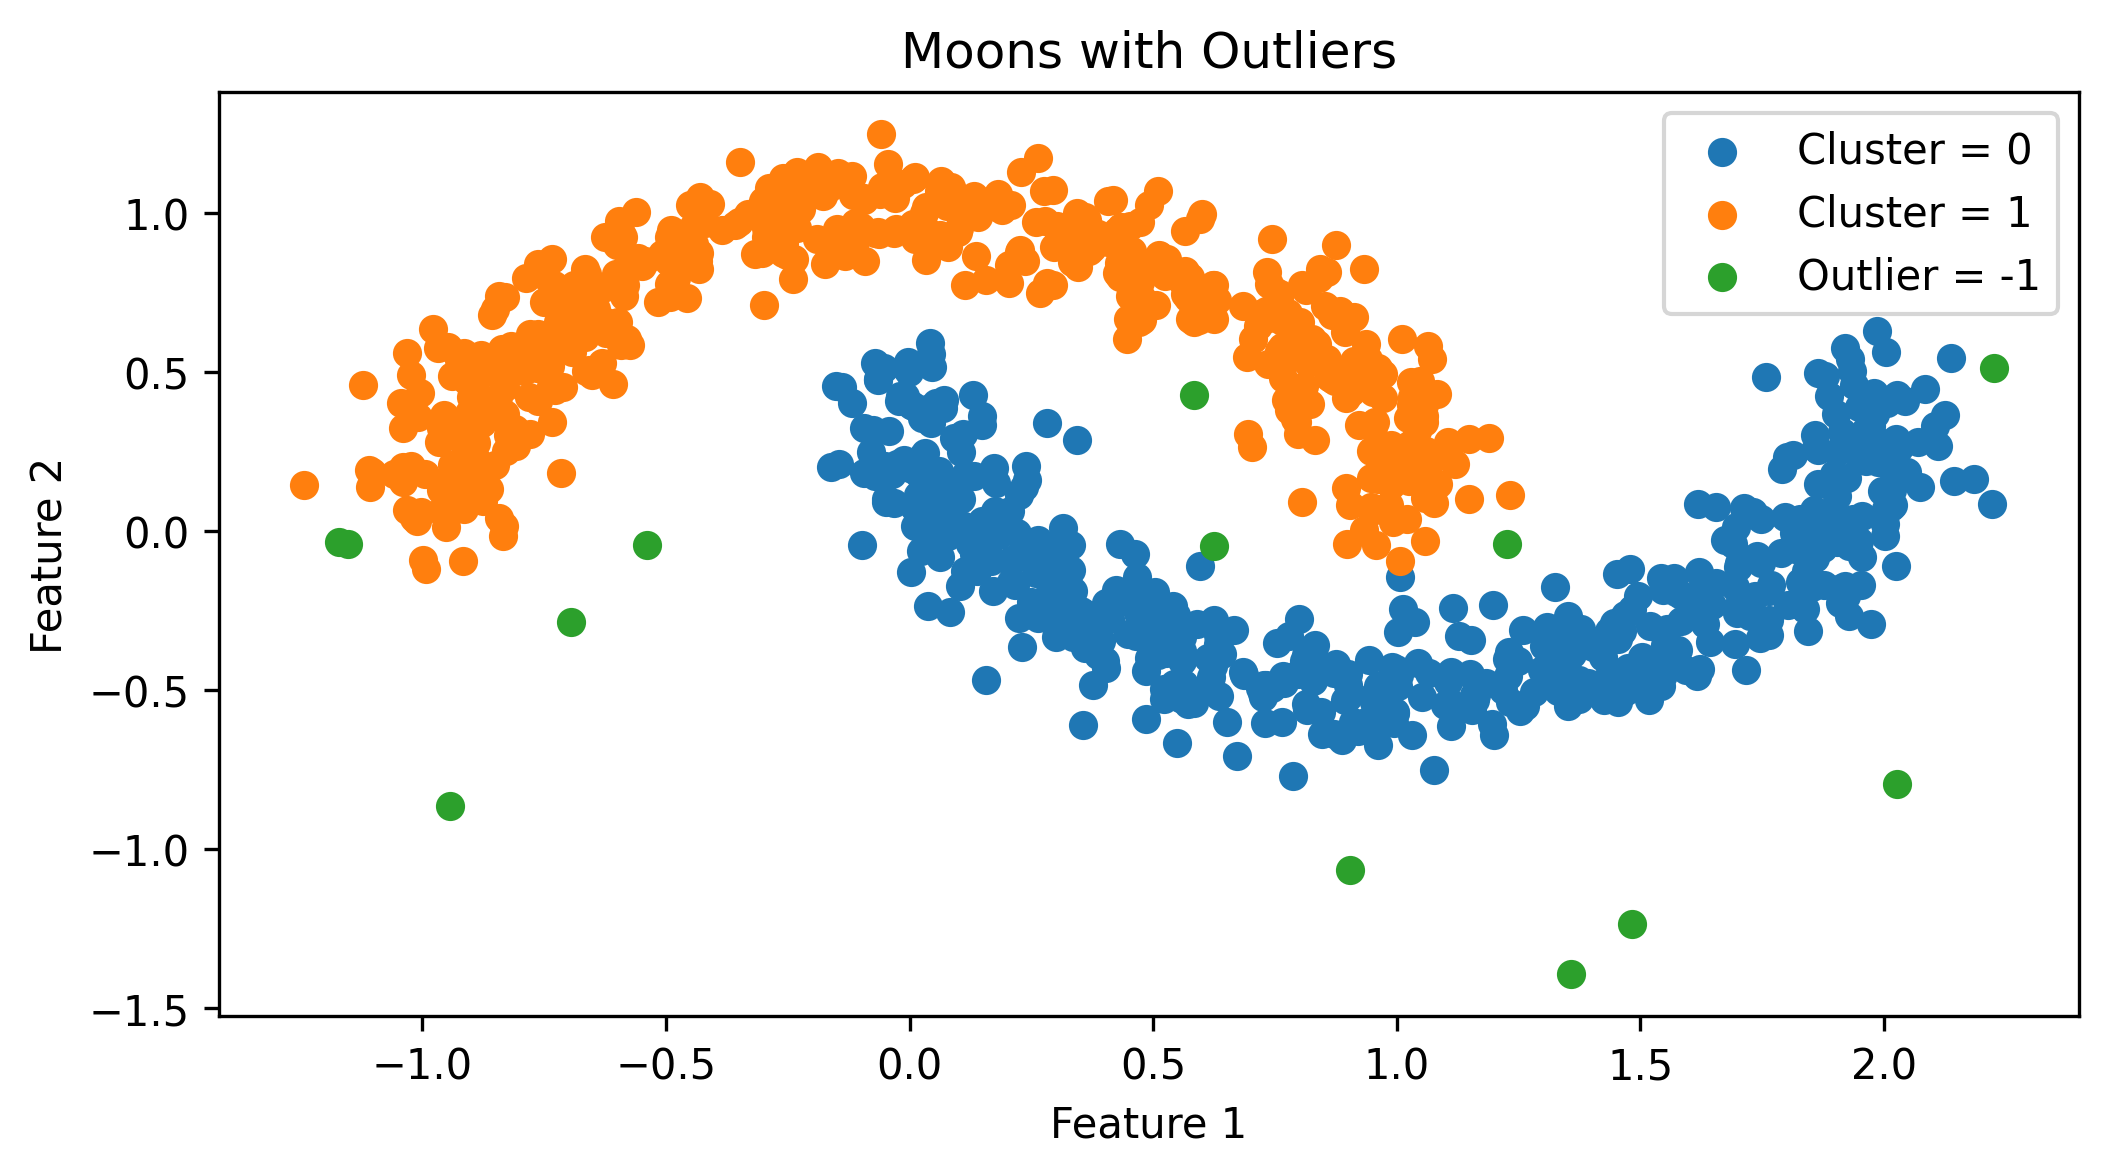
\includegraphics[scale=0.5]{notebooks/ML/img/dbscan_on_moons.png}
    \caption{DBSCAN Example}
\end{figure}

Para realizar esto, se siguen los siguientes pasos: 

\begin{enumerate}
    \item Encontrar todos aquellos puntos (\textit{core points}) que tengan más de \textit{MinNeighbor} vecinos a distancia menor de $\epsilon$. 
    \item Todos los \textit{core points} conexos serán asignados a un cluster. 
    \item Todos los \textit{non core points} serán asignados al cluster del \textit{core point} más cercano. El resto será considerado como \textit{outliers}. 
\end{enumerate}

Sea $C = \{ C_1 , \dots , C_{k} \}$ el número de clusters generados, el algoritmo anterior asegura la optimalidad del siguiente problema de optimización: 

\begin{equation*}
\begin{aligned}
\min_{C} \quad &|C| \\
\textrm{s.t.} \quad d(p,q) \leq \epsilon \hspace{0.5em} \forall &p,q \in C_i, \hspace{0.5em} \forall C_i \in C
\end{aligned}
\end{equation*}

\section{Principal Component Analysis (PCA)}

El análisis de componentes principales (PCA) es un método no supervisado de \textbf{reducción de dimensionalidad}. Consideremos la matriz con los datos $X \in \mathcal{M}_{N \times M}$, es decir, el dataset con $N$ filas y $M$ columnas. Se define la matriz de covarianza $K = (K_{ij})_{ij} \in \mathcal{M}_{M \times M}$ donde  
$$K_{ij} = \text{Cov}(X_i, X_j) = \mathbb{E}((X_i - \mathbb{E}(X_i))(X_j - \mathbb{E}(X_i)) = \mathbb{E}(X_iX_j) - \mathbb{E}(X_i)\mathbb{E}(X_j)$$

Cuando las features $i,j$ son linealmente independientes, entonces $K_{ij} = 0$. Si ambas crecen conjuntamente, entonces su covarianza será positiva y de caso contrario, será negativa. A continuación, se calculan los \textbf{valores y vectores propios}, es decir, los valores $(\lambda_i)_i$ y $(v_i)_i$ que cumplen para todo $i$ la relación 
$$
K v_i = \lambda v_i 
$$
Los componentes principales serán aquellos vectores propios $(v_i)_i$ cuyo valor propio asociado $(\lambda_i)_i$ es mayor, es decir, la \textbf{dirección de máxima varianza}. Para obtener la transformación de los datos a $k$ dimensiones, basta juntar los $k$ vectores propios con mayor valor propio en una matriz $V \in \mathcal{M}_{M \times k}$ y calcular 
$$ 
\hat{X} = XV \in \mathcal{M}_{N \times k}
$$
\begin{figure}[H]
    \center
    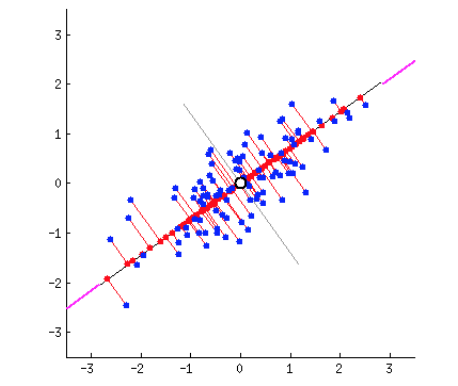
\includegraphics[scale=0.9]{notebooks/ML/img/pca_diagram.png}
    \caption{PCA Diagram}
\end{figure}
En problemas de clasificación o clustering, este enfoque puede ser útil para \textbf{visualizar etiquetas/clusters} en un gráfico de 2 o 3 dimensiones, o bien, puede ser utilizado para disminuir y condensar la información de un dataframe. 
\begin{figure}[H]
    \center
    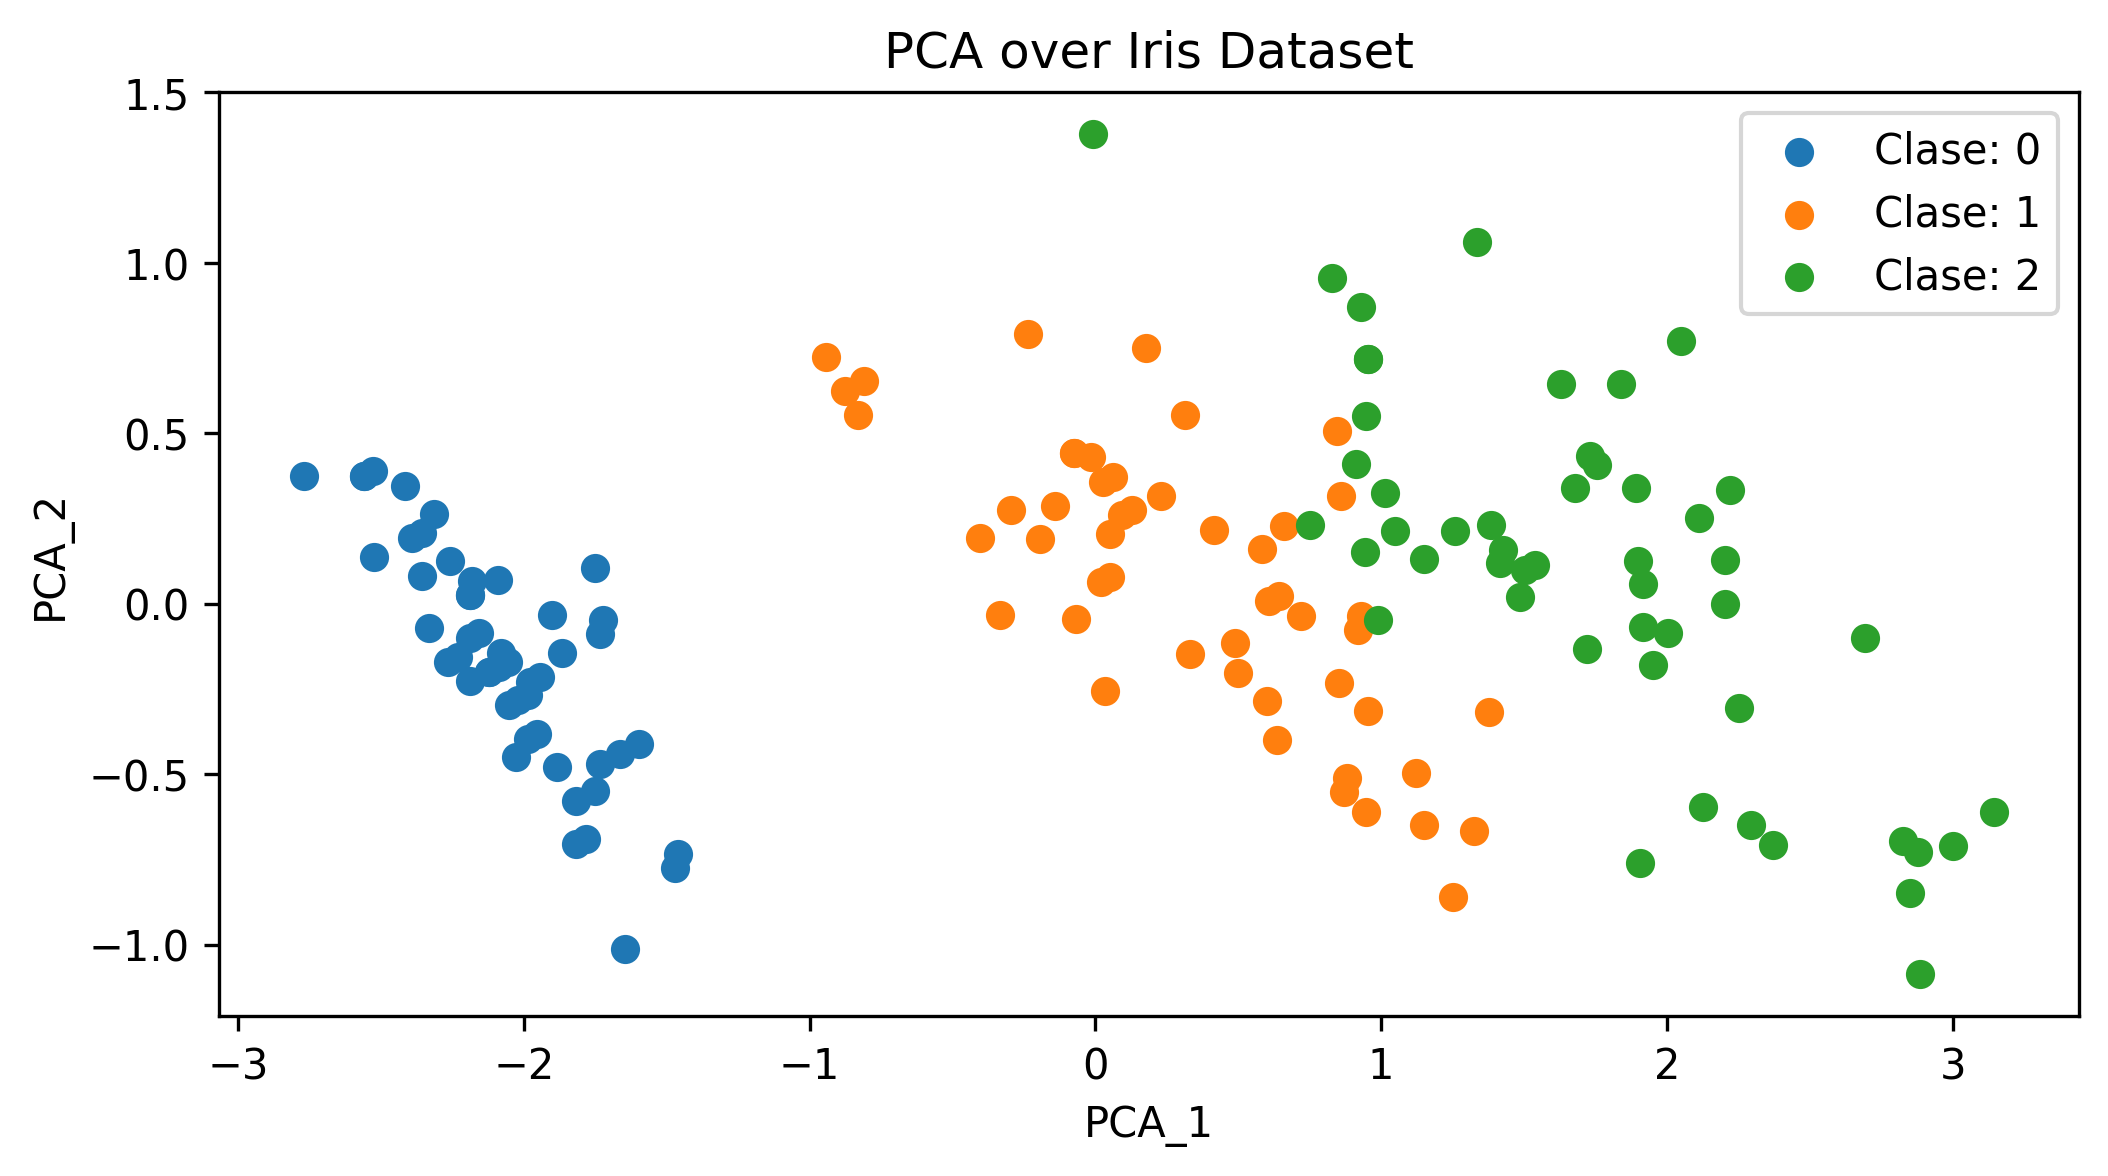
\includegraphics[scale=0.6]{notebooks/ML/img/pca_over_iris.png}
    \caption{PCA over Iris Dataset}
\end{figure}






